\chapter{Extensions}\label{sec:plugins}

La plupart des extensions décrites dans ce chapitre le sont également dans le Wiki. Les figures et les textes ont été copiés du Wiki mais adaptées pour être incluses dans des documents Latex (Miktex 2.0). 

\section{Généralités}

On peut étendre les fonctionnalités de \codeblocks en utilisant des extensions (ou plugins ou greffons, termes que l'on gardera parfois par commodité ci-dessous). Il y a généralement trois types de plugins :
\begin{description}
\item[Core plugins :] extensions développées et maintenues par l'équipe de base de \codeblocks.
\item[Contrib plugins :] extensions développées et maintenues par la communauté et reconnues comme étant appréciables. Elles sont donc intégrées dans le dépôt SVN de \codeblocks.
\item[3rd party plugins :] extensions développées et maintenues par la communauté mais pas (encore?) dans le dépôt de \codeblocks. Elles ont souvent leur propre dépôt ou ont été postées (incluant le code source) dans les forums.
\end{description}

\textbf{Si vous recherchez des plugins} :
\begin{enumerate}
\item Regardez dans la distribution officielle. Notez que l'installateur / "package manager" peut vous demander d'activer spécifiquement certains des plugins. Donc LISEZ attentivement.
\item Cherchez les annonces dans les forums, en particulier les forums de \url{https://forums.codeblocks.org/index.php/board,14.0.html}.
\item Il peut y avoir des informations sur le Wiki concernant d'autres plugins dans ses pages et ici : \url{https://wiki.codeblocks.org/index.php/Announcement_for_plugins/patches}.
\end{enumerate}

Pour les utilisateurs de Windows, le comportement par défaut de l'installateur est de ne \textbf{pas} installer les "contrib plugins". Vous devez manuellement cocher la case "contrib plugin" quand on vous proposera une sélection des composants à installer. Il n'y a pas franchement de moyen de les installer manuellement après coup.


\textbf{Si vous développez des plugins (ou extensions)} : Bien sûr, vous pouvez travailler sur des plugins/extensions comme bon vous semble, mais voici quelques suggestions:

\tab Annoncez-les sur le "plugin development board" dans les forums - en y incluant le code source (initial).

OU

\tab Créez votre propre page Web (ou utilisez une plate-forme de partage de fichiers) puis postez le lien d'accès vers les sources/binaires/svn sur le "plugin development board" dans les forums.

OU

\tab Créez un dépôt, par exemple sur BerliOS ou SourceForge, postez le lien d'accès vers les sources/binaires/svn sur le "plugin development board" dans les forums. \textbf{Veuillez noter :} C'est la meilleure façon de faire car les fichiers attachés dans nos forums peuvent être supprimés de temps en temps. Ce n'est donc pas très sûr de poster du code dans les forums.

ENFIN

\tab Entrez la description des plugins/extensions sur cette page.

\tab Annoncez le plugin en utilisant le formulaire sur \url{https://wiki.codeblocks.org/index.php/Template_for_plugin_announcement}

\begin{ASTYLE}
\section{Astyle}\label{sec:astyle}

Artistic Style est un indenteur de code source, un formateur de code source et un embellisseur de code source pour les langages de programmation C, C++, C\#. Il peut être utilisé pour sélectionner différents styles de règles de codage dans les \codeblocks.

\screenshot{astyle}{Formater votre code source}

Quand on indente un code source, nous en tant que programmeurs avons tendance à utiliser à la fois des espaces et des caractères de tabulations pour créer l'indentation souhaitée. De plus, certains éditeurs insèrent par défaut des espaces à la place des tabulations quand on appuie sur la touche Tab, alors que d'autres éditeurs ont la faculté de rendre d'embellir les lignes en ajoutant automatiquement des espaces en début de lignes, éventuellement en remplaçant dans ce code les tabulations utilisées jusqu'alors pour l'indentation par des espaces.

Comme le nombre de caractères affichés sur l'écran pour chaque caractère de tabulation change d'un éditeur à l'autre, un des problèmes courants auquel est confronté un programmeur qui passe d'un éditeur à un autre est qu'un code qui contient à la fois des espaces et des tabulations et qui était jusqu'à présent bien indenté, devient soudain difficile à regarder après le changement d'éditeur. Même si en tant que programmeur vous faites attention à n'utiliser QUE des espaces ou QUE des tabulations, récupérer un code de quelqu'un d'autre peut malgré tout être problématique.

C'est pour résoudre ce problème qu'Artistic Style a été créé - un filtre écrit en C++ qui ré-indente et reformate automatiquement les fichiers sources en C / C++ / C\#.

\hint{Quand vous copiez du code, par exemple depuis Internet ou d'un manuel, ce code sera automatiquement adapté aux règles de codage dans \codeblocks.}

\end{ASTYLE}

\begin{AUTOVERSIONING}
\section{AutoVersioning}\label{sec:autoversioning}

Une application de suivi de versions qui incrémente les numéros de version et de génération de votre application à chaque fois qu'un changement est effectué et l'enregistre dans un fichier \file{version.h} avec des déclarations de variables faciles à utiliser. Possède également une option pour proposer des changements dans un style à la SVN, un éditeur de schémas de versions, un générateur de journal des changements, et bien d'autres choses encore $\ldots$

\subsection{Introduction}

L'idée de développer l'extension AutoVersioning est venue lors du développement d'un logiciel en version pre-alpha qui exigeait des informations de version et d'état. Trop occupé par le codage, sans temps disponible pour maintenir la numérotation des versions, l'auteur a décidé de développer une extension qui puisse faire le travail avec aussi peu d'interventions que possible.

\subsection{Fonctionnalités}

Voici résumée la liste des fonctions couvertes par l'extension :

\begin{itemize}
\item Supporte C et C++.
\item Génère et incrémente automatiquement des variables de versions.
\item Éditeur de l'état du logiciel.
\item Éditeur de schéma intégré pour changer le comportement de l'auto incrémentation des valeurs de versions.
\item Déclaration des dates en mois, jour et année.
\item Style de version Ubuntu.
\item Contrôle des révisions Svn.
\item Générateur de journal des changements.
\item Fonctionne sous Windows et Linux.
\end{itemize}

\subsection{Utilisation}

Aller simplement dans le menu \menu{Projet,Autoversioning}. Une fenêtre popup comme celle-ci apparaîtra :

\figures[H][width=.45\columnwidth]{autoversion_configure}{Configuration d'un projet pour Autoversioning}

Quand on répond Oui au message de demande de configuration, la fenêtre principale de configuration d'AutoVersioning s'ouvre pour vous permettre de paramétrer les informations de version de votre projet.

Après avoir configuré votre projet pour la mise en version automatique, les paramètres entrés dans la boîte de dialogue de configuration sont enregistrées dans le fichier de projet et un fichier \file{version.h} est créé. Pour le moment, chaque fois que vous entrez dans le menu \menu{Projet,Autoversioning}, le dialogue de configuration qui apparaît vous permet d'éditer votre version de projet et les paramètres qui y sont liés, à moins que vous n'enregistriez pas les nouveaux changements effectués par l'extension dans le fichier de projet.

\subsection{Onglets de la boîte de dialogue}
\genterm{Valeurs de Version}

Ici vous entrez simplement les valeurs de version adéquates ou laissez l'extension Autoversioning le faire pour vous (voir \pxref{fig:autoversion_editor}).

\begin{description}
\item[Version Majeure] Incrémenté de 1 quand le numéro mineur atteint son maximum
\item[Version mineure] Incrémenté de 1 quand le numéro de génération dépasse la barrière de nombre de générations, la valeur étant remise à 0 quand il atteint sa valeur maximale.
\item[Numéro de génération] (également équivalent à numéro de Release) - Incrémenté de 1 chaque fois que le numéro de révision est incrémenté.
\item[Révision] Incrémenté aléatoirement quand le projet a été modifié puis compilé.
\end{description}

\screenshot{autoversion_editor}{Configuration des Valeurs de Version}

\genterm{État}

Quelques champs pour garder une trace de l'état de votre logiciel avec une liste de valeurs prédéfinies usuelles (voir \pxref{fig:autoversion_status}).

\begin{description}
\item[État du logiciel] Un exemple typique pourrait être v1.0 Alpha
\item[Abréviation] Idem à l'état du logiciel mais comme ceci : v1.0a
\end{description}

\screenshot{autoversion_status}{Configuration de l'État dans Autoversioning}

\genterm{Schéma}

Vous permet d'éditer comment l'extension incrémentera les valeurs de version (voir \pxref{fig:autoversion_scheme}).

\screenshot{autoversion_scheme}{Schéma de fonctionnement d'Autoversioning}

\begin{description}
\item[Valeur max pour numéro mineur] Valeur maximale que peut atteindre la valeur mineure. Une fois cette valeur atteinte, le numéro Majeur est incrémenté de 1 et à la compilation suivante le numéro mineur sera remis à 0.
\item[Nombre max de générations] Quand cette valeur est atteinte, le compteur sera remis à 0 à la génération suivante. Mettre à 0 pour ne pas limiter.
\item[Révision maximale] Comme Nombre max de générations. Mettre à 0 pour ne pas limiter.
\item[Révision aléatoire maximale] Les révisions s'incrémentent par un nombre aléatoire que vous décidez. Si vous mettez 1, les révisions s'incrémenteront évidemment par 1.
\item[Nombre de générations avant d'incrémenter Mineur] Après des changements de code et des compilations avec succès, l'historique des générations s'incrémente, et quand cette valeur est atteinte alors la valeur Mineure s'incrémente.
\end{description}

\genterm{Paramètres}

Ici vous pouvez entrer certains paramètres du comportement d'Autoversioning (voir \pxref{fig:autoversion_settings}).

\screenshot{autoversion_settings}{Paramètres d'Autoversioning}

\begin{description}
\item[Auto-incrémente Majeur et Mineur] Laisse l'extension incrémenter ces valeurs en utilisant le schéma. Si non coché, seuls les numéros de génération et de Révision s'incrémenteront.
\item[Créer des déclarations de dates] Crée des entrées dans le fichier \file{version.h} avec des dates et un style de version à la façon d'Ubuntu.
\item[Incrémentation automatique] Indique à l'extension d'incrémenter automatiquement dès qu'une modification est faite. Cette incrémentation interviendra avant la compilation.
\item[Langage de l'en-tête] Sélectionne le langage de sortie du fichier \file{version.h}
\item[Interroger pour incrémenter] Si Incrémentation automatique est coché, on vous interroge alors avant la compilation (si des changements ont été effectués) pour incrémenter les valeurs de version.
\item[Svn activé] Recherche dans le répertoire courant la révision Svn et la date puis génère les entrées correspondantes dans \file{version.h}
\end{description}

\genterm{Journal des changements}

Ceci vous permet d'entrer chaque changement effectué au projet afin de générer un fichier \file{ChangesLog.txt} (voir \pxref{fig:autoversion_changelog}).

\screenshot{autoversion_changelog}{Journal des changements d'Autoversioning}

\begin{description}
\item[Afficher les changements quand la version s'incrémente] Affichera une fenêtre popup d'édition de journal quand la version est incrémentée.
\item[Format du Titre] Un titre formaté avec une liste de valeurs prédéfinies.
\end{description}

\subsection{Inclusion dans votre code}

Pour utiliser les variables générées par l'extension faire simplement \codeline{\#include <version.h>}. Le code suivant est un exemple de ce qu'on peut faire :

\begin{lstlisting}
#include <iostream>
#include "version.h"

void main(){
    std::cout<<AutoVersion::Major<<endl;
}
\end{lstlisting}

\genterm{Sortie de version.h}

Le fichier d'en-tête généré. Voici un exemple sur un fichier en mode c++ :

\begin{lstlisting}
#ifndef VERSION_H
#define VERSION_H

namespace AutoVersion{

	//Date Version Types
	static const char DATE[] = "15";
	static const char MONTH[] = "09";
	static const char YEAR[] = "2007";
	static const double UBUNTU_VERSION_STYLE = 7.09;

	//Software Status
	static const char STATUS[] = "Pre-alpha";
	static const char STATUS_SHORT[] = "pa";

	//Standard Version Type
	static const long MAJOR = 0;
	static const long MINOR = 10;
	static const long BUILD = 1086;
	static const long REVISION = 6349;

	//Miscellaneous Version Types
	static const long BUILDS_COUNT = 1984;
	#define RC_FILEVERSION 0,10,1086,6349
	#define RC_FILEVERSION_STRING "0, 10, 1086, 6349\0"
	static const char FULLVERSION_STRING[] = "0.10.1086.6349";

}
#endif //VERSION_h
\end{lstlisting}

En mode C c'est la même chose qu'en C++ mais sans le namespace:

\begin{lstlisting}
#ifndef VERSION_H
#define VERSION_H

	//Date Version Types
	static const char DATE[] = "15";
	static const char MONTH[] = "09";
	static const char YEAR[] = "2007";
	static const double UBUNTU_VERSION_STYLE = 7.09;

	//Software Status
	static const char STATUS[] = "Pre-alpha";
	static const char STATUS_SHORT[] = "pa";

	//Standard Version Type
	static const long MAJOR = 0;
	static const long MINOR = 10;
	static const long BUILD = 1086;
	static const long REVISION = 6349;

	//Miscellaneous Version Types
	static const long BUILDS_COUNT = 1984;
	#define RC_FILEVERSION 0,10,1086,6349
	#define RC_FILEVERSION_STRING "0, 10, 1086, 6349\0"
	static const char FULLVERSION_STRING[] = "0.10.1086.6349";

#endif //VERSION_h
\end{lstlisting}

\subsection{Générateur de journal des changements}

Cette boîte de dialogue est accessible à partir du menu \menu{Projet, Journal des changements}. Également si la case "Afficher l'éditeur des changements quand la version s'incrémente" est cochée, une fenêtre s'ouvrira pour vous permettre d'entrer la liste des changements après une modification des sources du projet ou un évènement d'incrémentation (voir \pxref{fig:autoversion_changes}).

\screenshot{autoversion_changes}{Changements dans un projet}

\genterm{Résumé des Boutons}

\begin{description}
\item[Ajouter] Ajoute une ligne à la grille de données
\item[Éditer] Active les modifications de la cellule sélectionnée
\item[Supprimer] Supprime la ligne courante de la grille de données
\item[Enregistrer] Enregistre dans un fichier temporaire (\file{changes.tmp}) les données actuelles pour pouvoir effectuer plus tard les entrées dans le journal des changements
\item[Écrire] Entre la grille de données dans le journal des changements
\item[Annuler] Ferme simplement la boîte de dialogue sans rien faire d'autre
\end{description}

Voici un exemple de sortie générée par l'extension dans le fichier \file{ChangesLog.txt} :

\begin{lstlisting}
03 September 2007
   released version 0.7.34 of AutoVersioning-Linux

     Change log:
        -Fixed: pointer declaration
        -Bug: blah blah

02 September 2007
   released version 0.7.32 of AutoVersioning-Linux

     Change log:
        -Documented some areas of the code
        -Reorganized the code for readability

01 September 2007
   released version 0.7.30 of AutoVersioning-Linux

     Change log:
        -Edited the change log window
        -If the change log windows is leave blank no changes.txt is modified
\end{lstlisting}


\end{AUTOVERSIONING}

\begin{BROWSETRACKS}
\section{Browse Tracker}\label{sec:browsetracker}

Browse Tracker est une extension qui aide à naviguer parmi les fichiers récemment ouverts dans \codeblocks. La liste des fichiers récents est sauvegardée dans un historique. Le menu \menu{Vue,Suivi de Navigation,Tout Effacer} permet d'effacer l'historique.

Dans les différents \samp{onglets} vous pouvez naviguer entre les divers éléments des fichiers récemment ouverts en utilisant l'entrée de menu \menu{Vue,Suivi de Navigation,Aller en arrière/Aller en avant} ou en utilisant les raccourcis claviers Alt-Gauche/Alt-Droit. Le menu de suivi de navigation est également accessible dans les menus de contexte. Les marqueurs sont enregistrés dans un fichier de mise en page \file{\var{projectName}.bmarks}

Quand on développe du logiciel, on passe souvent d'une fonction à une autre implémentée dans différents fichiers. L'extension de suivi de navigation vous aidera dans cette tâche en vous montrant l'ordre dans lequel ont été sélectionnés les fichiers. Vous pouvez alors naviguer confortablement dans les différents appels de fonctions.

L'extension permet même de naviguer entre les marqueurs de chaque fichier de l'éditeur de \codeblocks. La position du curseur est mémorisée pour chacun des fichiers. Vous pouvez poser ces marqueurs en utilisant le menu \menu{Vue, Suivi de Navigation, Activer le marquage de navigation} ou en sélectionnant une ligne avec le bouton gauche de la souris. Une marque $\ldots$ est alors posée dans la marge gauche. Avec les menus \menu{Vue,Suivi de Navigation,Marque précédente/Marque suivante} ou les raccourcis Alt-up/Alt-down vous pouvez naviguer entre les différents marques posées dans un fichier. Si vous voulez naviguer dans un fichier avec des marques triées en fonction du numéro de lignes, choisissez simplement le menu \menu{Vue,Suivi de Navigation,Trier les marques de navigation}.

En choisissant \menu{Effacer la marque de navigation} le marqueur de la ligne sélectionnée est supprimé. Si un marqueur est posé sur une ligne, le fait d'appuyer pendant 1/4 de seconde sur le bouton gauche de la souris tout en appuyant sur la touche Ctrl effacera le marqueur de cette ligne. Avec le menu \menu{Effacer toutes les marques de navigation} ou avec un Ctrl-clic gauche sur toute ligne non marquée, vous remettez à 0 tous les marqueurs d'un fichier.

Le paramétrage de l'extension peut être configuré via le menu \menu{Paramètres,Éditeur,Browse Tracker}.

\hint{NdT : certains menus ou affichages ne sont pas traduits car l'auteur de l'extension n'a pas marqué certaines chaînes comme étant traduisibles}

\begin{description}
\item[Mark Style] (Styles des marques) Les marques de navigation sont affichées par défaut comme des $\ldots$ dans la marge. Avec le choix \menu{Book\_Marks} elles seront affichées en tant que marque par une flèche bleue dans la marge. L'option "hide" supprime l'affichage des marques.
\item[Toggle Browse Mark key] Les marques peuvent être activées ou supprimées soit par un simple clic avec le bouton gauche de la souris soit avec un clic-gauche tout en maintenant la touche Ctrl enfoncée.
\item[Toggle Delay] Durée pendant laquelle le bouton gauche de la souris est enfoncé pour entrer dans le mode de marquage de navigation.
\item[Clear All BrowseMarks] (Effacer toutes les marques) tout en maintenant enfoncée la touche Ctrl soit par simple clic soit par double-clic sur le bouton gauche de la souris.
\end{description}

La configuration de l'extension est enregistrée dans votre répertoire application data dans le fichier \file{default.conf}. Si vous utilisez la fonctionnalité des profils (ou personnalité) de \codeblocks la configuration est alors lue dans votre fichier \file{\var{personality}.conf}.







\end{BROWSETRACKS}

\begin{CODESNIPPETS}
\section{CodeSnippets}\label{sec:codesnippets}

L'extension CodeSnippets permet de structurer des modules de texte et des liens vers des fichiers en fonction de catégories dans une vue arborescente. Les modules sont utilisés pour stocker des fichiers fréquemment utilisés, des constructions de modules de texte, le tout géré depuis un endroit centralisé. Imaginez la situation suivante : Un certain nombre de fichiers source fréquemment utilisés sont stockés dans divers répertoires du système de fichiers. La fenêtre de CodeSnippets vous donne l'opportunité de créer des catégories et, à l'intérieur de ces catégories, des liens vers les fichiers requis. Avec cette fonctionnalité, vous pouvez contrôler l'accès aux fichiers indépendamment de l'endroit où ils sont stockés dans le système de fichiers, et vous pouvez rapidement naviguer entre ces fichiers sans avoir besoin de les chercher un peu partout dans le système.

\hint{Vous pouvez utiliser les variables \codeblocks ou les variables d'environnement dans les liens vers les fichiers comme \codeline{$(VARNAME)/name.pdf} pour paramétrer un lien dans le navigateur de CodeSnippets.}

La liste des modules de texte et des liens peut être enregistrée dans la fenêtre des CodeSnippets en cliquant sur le bouton droit de la souris et en sélectionnant \samp{Enregistrer l'index} depuis le menu de contexte. Le fichier \file{codesnippets.xml} qui est alors créé par cette procédure, se trouve dans le sous-répertoire \file{codeblocks} du répertoire \file{Documents and Settings\osp Application data} sous Win 7 (ou un chemin équivalent du profil de l'utilisateur, adapté à chaque OS). Sous Linux, cette information est enregistrée dans le sous-répertoire \file{.codeblocks} de votre répertoire HOME. Les fichiers de configuration de \codeblocks seront chargés au démarrage suivant. Si vous souhaitez enregistrer le contenu des CodeSnippets à un autre endroit, sélectionnez l'entrée \samp{Enregistrer l'index sous}. Pour charger ce fichier, sélectionnez \samp{Charger le fichier d'index} lors du démarrage suivant de \codeblocks ou incluez le répertoire dans les \samp{Paramètres} du menu de contexte de \samp{Répertoire des Snippets}. Les paramétrages sont enregistrés dans le fichier correspondant \file{codesnippets.ini} dans votre application data.

Pour inclure une catégorie, utilisez le menu \samp{Ajouter une sous-catégorie}. Une catégorie peut contenir des  Snippets (modules de texte) ou des Liens vers un fichier. Un module de texte est créé via la commande \samp{Ajouter un Snippet} depuis le menu de contexte. Le contenu est intégré dans le module de texte comme un \samp{Nouveau snippet} en sélectionnant un passage de texte dans l'éditeur de \codeblocks et en le glissant-déposant sur le module dont les propriétés s'affichent. En double-cliquant sur la nouvelle entrée ou en sélectionnant  \samp{Éditer le Texte} on en éditera le contenu.

\screenshot{edit_snippet}{Édition d'un module de texte}

La sortie d'un module de texte est gérée dans \codeblocks via la commande \samp{Appliquer} du menu de contexte ou en faisant un glisser-déposer dans l'éditeur. Sous Windows, le contenu d'un Snippet peut également être glissé-déposé dans d'autres applications. Dans le navigateur de CodeSnippets vous pouvez copier une sélection par glisser-déposer vers une catégorie différente.

De plus, les modules de texte peuvent être paramétrés par des variables \var{name} qui peuvent être accédées via  \codeline{$(name)} (voir \pxref{fig:edit_snippet}). Les valeurs des variables peuvent être récupérées dans un champ d'entrée si le module de texte est appelé via la commande du menu de contexte \samp{Appliquer}.

À côté des modules de texte, des liens vers des fichiers peuvent aussi être créés. Si, après avoir créé un module de texte, vous cliquez sur la commande \samp{Propriétés} du menu de contexte, vous pouvez alors sélectionner une cible de type lien en cliquant sur le bouton \samp{Lien cible}. Cette procédure convertira automatiquement le module de texte en un lien vers un fichier. Dans CodeSnippets, tous les modules de texte sont marqués par un symbole T, les liens vers un fichier par un symbole F et les urls par un symbole U. Si vous voulez ouvrir un fichier sélectionné (lien) dans la vue des codesnippets, sélectionnez tout simplement le menu de contexte \menu{Ouvrir le fichier} ou tout en maintenant enfoncée la touche \samp{Alt} effectuez un double-clic sur le fichier.

\hint{Vous pouvez même ajouter une url (comme https://www.codeblocks.org) dans les modules de texte. L'url peut être ouverte en utilisant le menu de contexte \menu{Ouvrir l'Url} ou en utilisant un glisser-déposer vers votre navigateur favori.}
%\hint{Si vous avez choisi la configuration \samp{L’ouvrir avec l’application associée} dans \menu{Paramètres,Environnement} pour la gestion de l’extension de fichiers, c’est l’application assignée par Windows pour cette extension de fichier qui sera utilisée (voir \pxref{sec:file_extension}).}

Avec un tel paramétrage, si vous ouvrez un lien vers un fichier pdf depuis la vue des codesnippets, un visualiseur de fichiers pdf sera automatiquement démarré. Cette méthode rend possible à l'utilisateur l'accès à des fichiers répartis un peu partout sur le réseau, comme des données, mises en forme, documentations etc., à l'aide des applications communes, simplement par le biais d'un lien. Le contenu des codesnippets est enregistré dans le fichier \file{codesnippets.xml}, la configuration est enregistrée dans le fichier \file{codesnippets.ini} de votre répertoire \file{application data}. Ce fichier ini contiendra, par exemple, le chemin du fichier \file{codesnippets.xml}.

\figures[hbt!][width=.4\columnwidth]{codesnippets}{Vue des CodeSnippets}

\codeblocks supporte l'utilisation de différents profils. Ces profils sont aussi nommés personnalités. En démarrant, avec l'option \opt{--personality=\var{profile}}, \codeblocks en ligne de commande vous créez ou utilisez un profil existant. Dans ce cas, le paramétrage ne sera pas enregistré dans le fichier \file{default.conf}, mais plutôt dans un \file{\var{personality}.conf} de votre répertoire \file{application data}. L'extension Codesnippets enregistrera alors ses paramètres dans un fichier \file{\var{personality}.codesnippets.ini}. Maintenant, si vous chargez un nouveau contenu \file{\var{name.xml}} dans les paramètres de codesnippets via \samp{Charger un fichier d'index}, ce contenu sera enregistré dans le fichier ini correspondant. L'avantage de cette méthode tient dans le fait que dans le cas où il y a différents profils, on peut gérer plusieurs configurations de modules de textes et de liens.

L'extension offre une fonction de recherche complémentaire pour naviguer dans les catégories et les Snippets. La façon de rechercher dans les Snippets, catégories ou Snippets et catégories peut s'ajuster. En entrant l'expression de recherche requise, l'entrée correspondante est automatiquement sélectionnée dans la vue. La \pxref{fig:codesnippets} affiche une fenêtre CodeSnippets typique.

%\figures[hbt!][width=.4\columnwidth]{codesnippets}{Vue des CodeSnippets}

\hint{Quand on utilise des modules de texte volumineux, le contenu de ces modules devrait être enregistré sous forme de fichiers via \samp{Convertir en lien vers fichier} de façon à réduire l'utilisation mémoire du système. Si vous supprimez un codesnippet ou un lien vers un fichier, il est en fait déplacé vers la corbeille (ou un répertoire \file{.trash}); si vous maintenez la touche Maj enfoncée, cet élément sera réellement détruit.}


\end{CODESNIPPETS}

\begin{CODECOMPLETION}
\section{Complétion de Code dans \codeblocks}\label{sec:codecompletion}

Deux extensions qui fournissent une fonctionnalité de complétion de code et navigation de classe. Ils ne sont pas compatibles entre-eux. Un seul des deux peut être activé.
 
\hint {Extrait de Wikipedia : La complétion de code intelligente est une fonction de complétion de code contextuelle dans certains environnements de programmation qui accélère le processus de codage des applications en réduisant les fautes de frappe et autres erreurs courantes. Les tentatives de complétion de code se font généralement par le biais de fenêtres pop-up d'autocomplétion pendant la saisie, l'interrogation des paramètres des fonctions, les conseils d'interrogation liés aux erreurs de syntaxe. La complétion de code intelligente et les outils connexes servent de documentation et à supprimer les ambiguïtés pour les noms de variables, les fonctions et les méthodes.}

\subsection{Extension de Complétion de Code }

\figures[H][width=.20\columnwidth]{Codecompletion_icon}{Icône de Complétion de Code}

\textbf{CodeCompletion} fourni un navigateur de symboles pour vos projets et une complétion de code interne à l'éditeur.
Lors de la complétion de code, on utilise un ensemble de symboles pour identifier le type associé avec les éléments suggérés ; ces symboles sont définis dans la table ci-dessous.

\figures[H][width=.75\columnwidth]{CodeCompletion}{Table de Complétion de Code}

Note : Ceci est un document utilisateur de l'extension Code Complétion.
Seuls les langages C/C++ sont supportés par cette extension (en l'état actuel)...

\subsection{Client Clangd pour CB}

Ce greffon fournit une fonctionnalité de complétion de code et navigation de classe par Clangd via LSP (Language Server Protocol).

La page d'accueil de l'extension est : \url{https://sourceforge.net/projects/cb-clangd-client/}

Le développeur principal est Pecan.

Le forum de discussion correspondant est : Code completion using LSP and clangd\newline
(\url{https://forums.codeblocks.org/index.php/topic,24357.msg166136.html})

Cette documentation est extraite du wiki : \url{https://wiki.codeblocks.org/index.php/CB_Clangd_Client}

\subsubsection{Qu'est-ce que Clangd}

clangd comprend votre code en C++ et ajoute des fonctions évoluées à votre éditeur :
\begin{itemize}[noitemsep]
\item complétion de code
\item erreurs à la compilation
\item aller à la définition
\item aller à l'implémentation
\item recherche de références
\end{itemize}
et bien plus.

clangd est un serveur de langage qui peut fonctionner avec votre éditeur via un greffon.\newline
\codeblocks vous apporte Clangd\_client en tant que greffon utile.

Clangd\_client améliore en outre le serveur clangd en fournissant :
\begin{itemize}[noitemsep]
\item appel d'astuces
\item définitions des fonctions
\item définitions des paramètres
\item fonction de positionnement sur précédent ou suivant
\item navigateur de symboles
\item aller au fichier
\item aller à la fonction
\item renommer des symboles
\end{itemize}

\textbf{NOTE :} Un \textbf{projet} \codeblocks \textbf{est nécessaire} pour le fonctionnement de Clangd\_client.

Clangd\_client ne fonctionne pas avec les parties de traduction en l'absence de projet.
							 
Un projet apporte les ressources nécessaires à l'interface entre l'Éditeur et le serveur Clangd.

\subsubsection{Configuration de clangd\_client}\label{sec:cfg_client}

Clangd\_client a besoin d'un exécutable tiers : clangd.

Voir \textbf{Windows : Compilateur Clangd/Installateur de Package LLVM} ci-dessous (\ref{sec:win_packages}) pour l'installer, ou \textbf{Linux : Processus d'installation de l'exécutable Clangd} (voir \ref{sec:linux_install})

Après l'installation avec succès de l'exécutable clangd, il faut faire ce qui suit :

\begin{itemize}[noitemsep]
\item Désactivez le greffon "CodeCompletion".
\item Allez dans \menu{Extensions, Gestion des extensions} et \textbf{désactivez} CodeCompletion.
\item Allez dans \menu{Extensions, Gestion des extensions} et \textbf{activez} Clangd\_client.
\end{itemize}
\textbf{Redémarrez \codeblocks.}

Configurez (ou vérifiez) dans \codeblocks là où est déclaré l'exécutable clangd :\par
\begingroup
\leftskip 6ex
Allez dans \menu{Paramètres, Éditeur, Clangd\_client, Parseur C/C++ (onglet)} et vérifiez l'emplacement de l'exécutable de clangd dans la boîte labellée "Spécifier l'exécutable clangd à utiliser".
\par
\endgroup

\subsubsection{Installation de Clangd\_client à partir des sources ou d'un binaire pré-généré}
\hint {Clangd\_client est maintenant inclus en tant que greffon contributeur dans les générations dites "Nightly".
Utiliser une génération "Nightly" est le moyen le plus simple pour mettre à jour clangd\_client.
Installer simplement la "Nightly" puis configurer comme décrit ci-dessous.\\
Voir les générations "Nightly" dans \url{https://forums.codeblocks.org/index.php/board,20.0.html}
}
\begin{enumerate}[noitemsep]
\item Installez LLVM ou Clangd.exe comme documenté dans la section ci-dessous de titre : \\
          \textbf{Installation sous Windows de l'exécutable Clangd} (voir \pxref{sec:win_install})

\item Désactivez le greffon Code completion comme suit :
    \begin{enumerate}[noitemsep]
    \item Ouvrez la Gestion des Extensions via le menu de \codeblocks \newline
          \menu{Menu Principal, Extensions, Gestion des extensions...} 
    \item Dans le dialogue de Gestion des extensions faire ce qui suit :
        \begin{enumerate}[noitemsep]
        \item Recherchez et sélectionnez le greffon "Code completion" à l'aide de son nom 
        \item Pressez sur le bouton "Désactiver" sur la droite proche du haut
        \item Si vous obtenez des erreurs ré-essayez.
        \end{enumerate}
    \end{enumerate}
	   
\item Installez le greffon Clangd-Client en utilisant une des options suivantes, qui sont documentées ci-dessous :
    \begin{enumerate}[noitemsep]
    \item Installer via la Gestion des extensions
    \item Installer à la main les fichiers du greffon
    \end{enumerate}
	
\item Configurez le greffon Clangd-Client en vue de son utilisation comme suit :
    \begin{enumerate}[noitemsep]
    \item Sélectionnez l'élément de menu de \codeblocks \menu{Paramètres, Éditeur...}
    \item Dans la liste sur la gauche cliquez/sélectionnez l'option "clangd\_client".
    \item Dans l'onglet "Parseur C/C++" modifiez "Spécifier l'exécutable clangd à utiliser" pour référencer le clangd.exe que vous avez installé via l'étape 1) ci-dessus. \\ 
     Quelques exemples de ce que cela pourrait être :
    \begin{verbatim}
    C:\msys64\clang64\bin\clangd.exe
    C:\msys64\clang32\bin\clangd.exe
    C:\LLVM\bin\clangd.exe
    C:\compilers\clang\clangd.exe
    \end{verbatim}
    \end{enumerate}
\end{enumerate}

\subsubsection{Suppression Manuelle du greffon Clangd-Client}

\begin{enumerate}[noitemsep]
\item Quittez \codeblocks \hspace{0pt} !
\item Si vous avez installé les fichiers à la main ou utilisé la Gestion des extensions, alors vous pouvez faire ce qui suit :
    \begin{enumerate}[noitemsep]
    \item Dans le répertoire \codeblocks \file{...\osp share\osp CodeBlocks}, supprimez le fichier \file{clangd\_client.zip}
    \item Dans le répertoire \codeblocks \file{...\osp share\osp CodeBlocks\osp plugins}, supprimez le fichier \file{clangd\_client.dll}
    \end{enumerate}
\item Si vous avez installé via la Gestion des extensions, alors vous pouvez supprimer les fichiers avec les commandes suivantes :
    \begin{enumerate}[noitemsep]
    \item del \file{\%APPDATA\%\osp CodeBlocks\osp share\osp codeblocks\osp plugins\osp clangd\_client.dll}
    \item del \file{\%APPDATA\%\osp CodeBlocks\osp share\osp codeblocks\osp clangd\_client.zip}
    \end{enumerate}
\item Si vous voulez ré-utiliser l'ancien "code completion", pensez à réactiver le greffon
\end{enumerate}


\subsubsection{Windows : Installation sous Windows de l'exécutable Clangd}\label{sec:win_install}

Il y a 3 options principales pour installer clangd.exe:
\begin{enumerate}[noitemsep]
\item Installer un compilateur LLVM.
\item Extraire à la main les fichiers nécessaires du compilateur LLVM.
\item Installer un package Clangd pour le compilateur Windows que vous utilisez, s'il est disponible.
\end{enumerate}

Les étapes pour effectuer ces trois options sont détaillées ci-dessous.

\paragraph*{Windows : Installer le compilateur LLVM}\label{sec:llvm_install}

\begin{enumerate}[noitemsep]
\item Téléchargez le dernier (non RC/Beta) exécutable LLVM Windows pour votre OS (Win32 ou Win64) depuis la page de téléchargement Github de LLVM : \newline
      \url{https://github.com/llvm/llvm-project/releases} \newline

  Depuis Janvier 2022 les noms des fichiers Windows sont :
  \begin{verbatim}
     LLVM-<version>-win64.exe
     LLVM-<version>-win32.exe
  \end{verbatim}
  où \file{<version>} est la version de LLVM, comme 13.0.0 ou 13.0.1.\\

\item Lancez \file{LLVM-<version>-win<xx>.exe} que vous avez téléchargé pour installer le compilateur LLVM.
\end{enumerate}

\paragraph*{Windows : Extraction Manuelle des fichiers du compilateur LLVM}\label{sec:llvm_extract}
\begin{enumerate}[noitemsep]
\item Téléchargez le dernier (non RC/Beta) exécutable LLVM Windows pour votre OS (Win32 ou Win64) depuis la page de téléchargement Github de LLVM : \newline
      \url{https://github.com/llvm/llvm-project/releases} \newline

  Depuis Janvier 2022 les noms des fichiers Windows sont :
  \begin{verbatim}
     LLVM-<version>-win64.exe
     LLVM-<version>-win32.exe
  \end{verbatim}
  où \file{<version>} est la version de LLVM, comme 13.0.0 ou 13.0.1.\\

\item Dézippez le fichier \file{LLVM-<version>-win<xx>.exe} que vous avez téléchargé avec 7ZIP ou votre programme ZIP préféré dans un sous-répertoire
\item Créez un nouveau répertoire pour y placer clangd.exe et ses dll's
\item Copiez les fichiers suivants dans ce nouveau répertoire à partir du répertoire où a été dézippé LLVM :
    \begin{verbatim}
    bin\clangd.exe
    bin\msvcp140.dll
    bin\vcruntime140.dll
    bin\vcruntime140\_1.dll
    \end{verbatim}
\end{enumerate}

\paragraph*{Windows : Compilateur Clangd/Installateur de Package LLVM}\label{sec:win_packages} \hspace{0pt} \\
   En raison du nombre de compilateurs différents disponibles pour Windows, tous ces compilateurs n'auront pas forcément à la fois 
   les fichiers requis pour Clang ou LLVM.

   Si vous voulez installer un (ou des) package(s) spécifique(s) pour votre compilateur Windows, celui que vous avez, afin d'y utiliser le fichier clangd.exe, veuillez suivre les instructions ci-dessous pour le compilateur spécifique que vous avez installé :

   \subparagraph*{MSYS2 Compiler - MinGW64} \hspace{0pt} \\
   Il y a 2 options principales pour installer clangd.exe :
   \begin{enumerate}[noitemsep]
   \item La première option afin de minimiser l'espace disque est d'installer les "Clang extra tools" en utilisant l'un des packages suivants :       
        {\footnotesize
        \begin{longtable}{|l|l|}\hline
        \textbf{Package}                            & \textbf{Exécutable Clangd}    \\ \hline
%        \endhead   % To repeat the title line, if needed
        mingw-w64-clang-x86\_64-clang-tools-extra   & clang64/bin/clangd.exe        \\
        mingw-w64-x86\_64-clang-tools-extra         & mingw64/bin/clangd.exe        \\ \hline
%        \caption{Msys2 - Clang Extra Packages pour MinGW64}
        \end{longtable}
        \par}
 
        Pour intaller le package faire ce qui suit :
        \begin{enumerate}[noitemsep]
        \item Ouvrir un shell bash via msys2.exe 
        \item Y lancer la commande suivante : \newline
              \file{pacman -S <Package name in the table above>} \newline
        \end{enumerate}

       "OU" \newline

    \item La seconde option est d'installer la version complète des "Clang tool chain" comme suit :
        \begin{enumerate}[noitemsep]
        \item Ouvrir un shell bash via msys2.exe 
        \item Y lancer la commande suivante : \newline
              \file{pacman -S mingw-w64-clang-x86\_64-toolchain}
        \end{enumerate}
    \end{enumerate}

    \subparagraph*{MSYS2 Compiler - MinGW32} \hspace{0pt} \\
     Il y a 2 options principales pour installer clangd.exe :
     \begin{enumerate}[noitemsep]
     \item La première option afin de minimiser l'espace disque est d'installer les "Clang extra tools" en utilisant l'un des packages suivants :\\
        {\footnotesize
        \begin{longtable}{|l|l|}\hline
        \textbf{Package}                            & \textbf{Exécutable Clangd}    \\ \hline
%        \endhead   % To repeat the title line, if needed
        mingw-w64-clang-i686-clang-tools-extra      & clang32/bin/clangd.exe        \\
        mingw-w64-i686-clang-tools-extra            & mingw32/bin/clangd.exe        \\ \hline
%        \caption{Msys2 - Clang Extra Packages pour MinGW32}
        \end{longtable}
        \par}

        Pour installer le package faire ce qui suit :
        \begin{enumerate}[noitemsep]
        \item Ouvrir un shell bash via msys2.exe
        \item Y lancer la commande suivante : \newline
              \file{pacman -S <Package name in the table above>}\newline
        \end{enumerate}

        "OU" \newline

     \item La seconde option est d'installer la version complète des "Clang tool chain" comme suit :
        \begin{enumerate}[noitemsep]
        \item Ouvrir un shell bash via msys2.exe
        \item Y lancer la commande suivante : \newline
              \file{pacman -S mingw-w64-clang-i686-toolchain}
        \end{enumerate}
    \end{enumerate}

\rule{\textwidth}{0.4pt} \\    
    \textbf{Notes vues sur le forum \codeblocks afin d'éviter un mélange d'exécutables gcc/clangd incompatibles.}\\
\rule{\textwidth}{0.4pt} \\  
    {\small \url{https://forums.codeblocks.org/index.php/topic,24357.msg169412.html#msg169412}}

    \textbf{Ne mélangez surtout pas mingw64 avec clang64.}
    
    Si vous utilisez la version gcc de msys2, (compilateurs dans le répertoire "\file{msys64\osp mingw64\osp bin}"), vous devriez utiliser "\file{mingw-w64-x86\_64-clang-tools-extra}", (le fichier \file{clangd.exe} est dans le répertoire "\file{msys64\osp mingw64\osp bin}") soit le même répertoire que votre \file{gcc.exe}.
 
	Si vous utilisez la version complète de "clang tool chain", (le répertoire "\file{msys64\osp clang64\osp bin}"), vous devriez utiliser "\file{mingw-w64-clang-x86\_64-clang-tools-extra}".

	J'ai trouvé que j'avais fait une grosse erreur : c'est que j'utilisais la chaine d'outils gcc de "\file{msys64\osp mingw64\osp bin}", mais que j'utilisais le \file{clangd.exe} de "\file{msys64\osp clang64\osp bin}".
    Le résultat, c'est que j'obtenais un grand nombre de messages de diagnostiques et d'erreurs de LSP.\\
    Par chance, j'en ai trouvé la raison, et corrigé ce problème. En espérant que cela serve à d'autres.
%}

\subsubsection{Linux : Processus d'installation de l'exécutable Clangd}\label{sec:linux_install}

NOTE : Le greffon Clangd\_client a besoin d'un exécutable clangd en version 13 ou supérieure.

Vérifiez votre version actuelle de clangd en exécutant \file{clangd --version}.\newline
Si le numéro de version est inférieur à 13 vous devrez installer une version plus récente.

Voir \url{https://clangd.llvm.org/installation.html}

L'installation d'un package clangd vous donnera couramment une version légèrement plus ancienne.\newline
Testez cela en exécutant \file{apt-get install --dry-run clangd}

Depuis le 16/11/2022, c'est la version 10 de clangd qui sera installée.\newline
Si le numéro de version de clangd affiché est inférieur à 13, vous devrez installer une version spécifique comme suit :

Installez un package "release" (\textit{doit être en version 13 ou supérieure}):

\file{sudo apt-get install clangd-13} (\textit{Doit être en version 13 ou supérieure}).

Cela installera clangd dans \file{/usr/bin/clangd-13}.

Vous pouvez maintenant configurer le greffon clangd\_client en suivant les instructions précédentes dans \textbf{Configuration de clangd\_client} (voir \pxref{sec:cfg_client}

Si vous préférez installer entièrement le package LLVM/Clang, parce que c'est ce que vous voulez, il existe un script automatique d'installation disponible pour vous installer LLVM.

Pour installer la dernière version stable : voir \url{https://apt.llvm.org/}, "Automatic installation script".
Notez que dans ce script, vous devrez spécifier le numéro de version voulu.
\end{CODECOMPLETION}

\begin{CSCOPE}
\section{CScope}\label{sec:cscope}

Ce paragraphe est une extraction traduite du contenu de \href{https://wiki.codeblocks.org/index.php/Cscope_plugin}{"cscope plugin"} dans le wiki.

\subsection{Généralités}

Ce greffon intègre les fonctionnalités de recherche dans un code de \href{https://cscope.sourceforge.net/}{Cscope} dans \codeblocks (une version pour Windows est disponible dans \href{https://code.google.com/p/cscope-win32/}{Cscope-win32}). Cscope est particulièrement utile sur de gros projets, et peut rechercher :

\begin{itemize}[noitemsep]
\item toutes les références à un symbole
\item les définitions globales
\item les fonctions appelées par une fonction
\item les fonctions appelant une autre fonction
\item des chaînes de texte
\item un modèle d'expression régulière
\item un fichier
\item des fichiers incluant un autre fichier
\end{itemize}

Bien que l'analyseur syntaxique de Cscope soit ciblé sur du C, il conserve suffisamment de flexibilité pour fournir ses fonctionnalités sur du code en C++ (et Java).

\subsection{Installation de CScope}

Ces instructions sont pour \codeblocks, Version de SVN \textgreater  11828

\subsubsection{Linux}

Sous Linux, installer cscope devrait être aussi simple que d'appeler votre gestionnaire de "packages" préféré pour installer cscope. \codeblocks devrait trouver l'exécutable par défaut. S'il ne peut pas trouver l'exécutable de cscope, veuillez le configurer dans \menu{Paramètres,Environnement,CScope}. Vous pouvez trouver le chemin vers l'exécutable cscope en tapant \codeline{locate cscope} dans votre terminal préféré.

\subsubsection{Windows}

Il est assez difficile de trouver un binaire précompilé de cscope sous Windows. La solution la plus simple est d'installer \href{https://www.msys2.org/}{msys2}. Suivez les instructions sur le site web \cite{url:msys2} pour installer msys2. Après avoir installé et mis à jour comme décrit, ouvrez le terminal de msys et tapez \codeline{pacman -S cscope}. Ceci installera cscope depuis le dépôt global de "packages".

Maintenant vous devez configurer \codeblocks:

\begin{itemize}[noitemsep]
\item Ouvrir \codeblocks
\item \menu{Paramètres,Environnement,CScope}
\item Cliquer sur le bouton ... avec 3 points
\item Rechercher l'exécutable cscope.exe. Il est probablement situé dans \newline
    \file{REPERTOIRE\_INSTALLATION\_DE\_MSYS2\osp usr\osp bin\osp cscope.exe}
\item Fermer le dialogue via OK
\item Maintenant vous devriez pouvoir utiliser les fonctions de cscope dans \codeblocks (par ex. "Rechercher les fonctions appelant XXXX").
\end{itemize} 

\end{CSCOPE}

\begin{DOXYBLOCKS}
\section{Doxyblocks}\label{sec:doxyblocks}

DoxyBlocks est une extension pour \codeblocks qui intègre doxygen dans l'IDE. Il vous permet de créer de la documentation, insérer des blocs de commentaires et de lancer des documents HTML ou CHM. Il fournit également la configuration de quelques-uns des paramètres les plus communément utilisés at un accès à doxywizard pour obtenir une configuration plus détaillée.

Les paramètres de la barre d'outils de DoxyBlocks ont la signification suivante :

\begin{description}
\item[
\includegraphics{Doxywizard}] Lancer doxywizard. Ctrl-Alt-D
\item[
\includegraphics{Extract}] Extraire la documentation du projet courant. Ctrl-Alt-E
\item[
\includegraphics{Comment_block}] Insère un bloc de commentaires sur la ligne courante. De plus, DoxyBlocks essaiera de façon intelligente de lire si une méthode existe dans la ligne où le commentaire est en train d'être ajouté. Ctrl-Alt-B

\begin{lstlisting}
/** \brief
 *
 * \param bar bool
 * \return void
 *
 */    
void MyClass::Foo(bool bar)
{
    fooBar(bar);
}
\end{lstlisting}

\item[
\includegraphics{Comment_line}] Insère une ligne de commentaire à la position actuelle du curseur. Ctrl-Alt-L
\begin{lstlisting}
void MyClass::Foo(bool bar)
{
    fooBar(bar); /**<  */
}
\end{lstlisting}

\item[
\includegraphics{Html}] Affiche la documentation HTML générée. Ctrl-Alt-H
\item[
\includegraphics{Chm}] Affiche la documentation CHM (Help) générée. Ctrl-Alt-C
\item[
\includegraphics{Configure}] Ouvre les préférences de DoxyBlocks. Ctrl-Alt-P
\end{description}

Doxyblocks ne peut travailler que si doxygen est installé sur votre système. Vous avez besoin au moins des exécutables de doxygen et de doxywizard (disponibles dans la distribution officielle de doxygen sur \url{http://www.doxygen.nl/}). En option, vous pouvez avoir l'exécutable "dot" du package graphviz (voir \url{https://graphviz.gitlab.io/}. Sous Windows, le compilateur d'aide (hhc) peut également être utilisé les fichiers de type chm.

\genterm{Notes}
\begin{description}
\item Dans les préférences, vous avez une case à cocher qui autorise ou pas DoxyBlocks à \textbf{écraser le fichier doxyfile}. Par défaut, si un doxyfile existe déjà il ne sera pas écrasé pour protéger de divers changements qui auraient pu être faits en dehors de DoxyBlocks. Néanmoins ce comportement empèche aux changements faits par DoxyBlocks lui-même d'être écrits dans le doxyfile existant.
\item Si un champ de texte des "Préférences" est vide, DoxyBlocks assumera que l'exécutable correspondant est disponible quelquepart via votre variable d'environnement path. Vous pouvez utiliser des macros telles que \$(CODEBLOCKS) dans votre path et elles seront automatiquement étendues.
\item [OUTPUT\_DIRECTORY] Utilisé pour spécifier le chemin de base (relatif ou absolu) ou sera enregistrée la documentation générée. Si un chemin relatif est entré, il sera en relatif par rapport à l'emplacement d'où doxygen a été lancé. Si laissé en blanc, c'est le répertoire courant qui sera utilisé. Doxyblocks utilisera le nom de chemin entré ici pour créer un répertoire relatif au \codeline{<rep. projet>}. Ceci vout permet de créer des répertoire doxygen différents pour des projets inclus dans un même répertoire, ou simplement utiliser un nom de répertoire différent. Si le champ est laissé en blanc, les documents seront créés dans "\codeline{<rep. projet>/doxygen}". Entrer les noms de répertoires sans points, ni séparateurs de tête, ni nom de volume, etc. DoxyBlocks effectue la validation sur le nom de chemin et supprime les caractères en trop.
\begin{verbatim}
Exemples:
[blanc]           -> <répertoire projet>/doxygen.
"docs"            -> <répertoire projet>/docs.
"docs/sub1/sub2"  -> <répertoire projet>/docs/sub1/sub2.
"doxygen/docs"    -> <répertoire projet>/doxygen/docs.
\end{verbatim}
\item [OUTPUT\_LANGUAGE]  Utilisé pour spécifier dans quelle langue sera générée la documentation par doxygen. Doxygen utilisera cette information pour générer toutes les sorties constantes dans la langue adéquate. La langue par défaut est l'anglais. D'autres langues sont supportées. 
\item D'autres informations dans les fichiers d'aide de doxygen
\end{description}
\end{DOXYBLOCKS}

\begin{EDITORTWEAKS}
\section{Extension Editor Tweaks}\label{sec:editor_tweaks}

Le plugin EditorTweaks (modifications d'édition) apporte plusieurs fonctionnalités différentes. Sur une base de travail fichier à fichier, il contrôle :

\begin{itemize}[noitemsep]
\item le repliement de mots ;
\item la numérotation des lignes ;
\item l'interprétation de la touche tab (caractère de tabulation ou espaces) ;
\item le nombre de caractères espace remplaçant la touche tab ;
\item les caractères de fin de ligne (carriage-return + linefeed; carriage-return; linefeed) ;
\item la visualisation des caractères de fin de ligne ;
\item sur demande, la suppression des espaces blancs en fin de ligne ;
\item sur demande, la synchronisation des caractères de fin de ligne ;
\item la suppression de la touche d'insertion.
\end{itemize}

Depuis la fusion avec le plugin "Aligner", il peut rendre des sections de code plus lisibles en les alignant sur un caractère spécifique.\newline
Par exemple, aligner sur le caractère "=" dans :

\begin{lstlisting}
int var = 1;
int longVarName = 2;
int foobar = 3;
\end{lstlisting}

se traduira par :

\begin{lstlisting}
int var         = 1;
int longVarName = 2;
int foobar      = 3;
\end{lstlisting}

\end{EDITORTWEAKS}

\begin{ENVVAR}
\section{Extension Variables d'Environnement}\label{sec:EnvVar_Plugin}

D'après le wiki de \codeblocks. Voir aussi la \pxref{sec:EnvVars_Cfg}.

L'extension \textbf{Éditeur de variables d'environnement} permet de définir des variables d'environnement du système dans le cadre de \codeblocks.\newline
L'utilisateur peut avoir plusieurs ensembles qui contiennent 1..n variables d'environnement.\newline
L'utilisateur peut passer d'un ensemble à l'autre via la boîte de dialogue de configuration des variables d'environnement.\newline
En outre, l'extension EnvVars apporte une option aux projets (dans la configuration du projet) pour appliquer un ensemble EnvVar particulier à activer (et à utiliser pendant la compilation).

La boîte de dialogue permettant de modifier les ensembles se trouve dans \menu{Paramètres,Environnement,Variables d'environnement}.\newline
La boîte de dialogue permettant de choisir l'ensemble actif pour le projet en cours se trouve dans \menu{Projet,Propriétés,Options EnvVar}.\newline

\textbf{Script binding}

Cette extension apporte sa fonctionnalité via un "squirrel binding" : 

{\footnotesize
\begin{longtable}{|l|l|l|l|}\hline
\textbf{Valeur de retour}&\textbf{Nom}      &\textbf{Arguments}     &\textbf{Remarques}                     \\ \hline
\endhead    % Pour répéter la ligne de titre si besoin
wxArrayString   &EnvvarGetEnvvarSetNames    &                       &Retourne tous les ensembles            \\
                &                           &                       &envvar disponibles                     \\ \hline
wxString        &EnvvarGetActiveSetName     &                       &Retourne le nom de l'ensemble          \\
                &                           &                       &actif courant                          \\
                &                           &                       &(depuis config, /active\_set)          \\ \hline
wxArrayString   &EnvVarGetEnvvarsBySetPath  &const wxString         &Retourne les envvars d'un              \\
                &                           &set\_name              &chemin d'ensembles envvars             \\
                &                           &                       &dans la config                         \\ \hline
bool            &EnvvarSetExists            &const wxString         &Vérifie si un ensemble d'envvars       \\
                &                           &set\_name              &existe effectivement dans la config    \\ \hline
bool            &EnvvarSetApply             &const wxString\&       &Applique un ensemble envvar            \\
                &                           &set\_name,             &spécifique de la config                \\
                &                           &bool even\_if\_active  &(sans interaction de l'IU)             \\ \hline
void            &EnvvarSetDiscard           &const wxString         &Ignore un ensemble envvar              \\
                &                           &                       &spécifique de la config                \\
                &                           &                       &(sans interaction de l'IU)             \\ \hline
bool            &EnvvarApply                &const wxString key,    &Applique un envvar spécifique          \\
                &                           &const wxString value   &                                       \\ \hline
bool            &EnvvarDiscard              &const wxString key     &Ignore un envvar                       \\ \hline
\caption{Squirrel binding}
\end{longtable}
\par}

\textbf{NOTE} : Les arguments "value" sont automatiquement générés à partir des macros. Vous n'avez pas besoin d'appeler ReplaceMacros() sur ceux-ci.

Beaucoup d'autres fonctions de script sont disponibles. Regardez dans \url{https://wiki.codeblocks.org/index.php/Scripting_commands}

\textbf{Exemple}

Dans les fenêtres des étapes de post ou pré-génération :
\begin{lstlisting}
[[EnvvarApply(_("test"),_("testValue"));]]
echo %test%
\end{lstlisting}


\end{ENVVAR}

\begin{FILEMANAGER}
\section{Extensions FileManager et PowerShell}\label{sec:file_explorer}

L'explorateur de fichiers \pxref{fig:file_explorer} est inclus dans l'extension FileManager, et se trouve dans l'onglet  \samp{Fichiers}. L'aspect de File Explorer est montré à la \pxref{fig:file_explorer}.

En haut vous trouverez le champ d'entrée du chemin. En cliquant sur le bouton à l'extrémité de ce champ, la flèche vers le bas listera un historique des entrées précédentes dans lesquelles on peut naviguer à l'aide d'une barre de défilement. La flèche vers le haut à droite du champ déplace d'un cran vers le haut dans la structure des répertoires.

Dans le champ \samp{Joker} vous pouvez entrer un filtre de visualisation pour l'affichage des fichiers. En laissant vide ce champ ou en y entrant \codeline{*} vous afficherez tous les fichiers. En y entrant \codeline{*.c;*.h} par exemple, vous n'afficherez que les fichiers sources en C et les fichiers d'en-têtes (headers). Ouvrir la flèche du bas, affiche de nouveau la liste des dernières entrées.

\figures[hbt!]{file_explorer}{Le gestionnaire de fichiers}

Appuyer sur la touche Maj tout en cliquant, sélectionne un groupe de fichiers ou de répertoires, alors qu'appuyer sur la touche Ctrl tout en cliquant sélectionne des fichiers multiples ou des répertoires séparés.

Les opérations suivantes peuvent être obtenues via le menu de contexte si un ou plusieurs répertoires ont été sélectionnés dans l'Explorateur de Fichiers :

\begin{description}
\item[Make Root] défini le répertoire courant comme répertoire de base.
\item[Ajouter aux favoris] configure un marqueur pour ce répertoire et l'enregistre dans les favoris. Cette fonction permet de naviguer rapidement entre des répertoires fréquemment utilisés ou encore sur des disques réseau.
\item[Nouveau Fichier] crée un nouveau fichier dans le répertoire sélectionné.
\item[Nouveau Répertoire] crée un nouveau sous répertoire dans le répertoire sélectionné.
\end{description}

Les opérations suivantes peuvent être obtenues via le menu de contexte si un ou plusieurs fichiers ou même un ou plusieurs répertoires ont été sélectionnés dans l'Explorateur de Fichiers :

\begin{description}
\item[Dupliquer] copie un fichier/répertoire et le renomme.
\item[Copier vers] ouvre une boîte de dialogue pour entrer un répertoire cible dans lequel on copiera les fichiers/répertoires.
\item[Déplacer vers] déplace la sélection vers un autre endroit.
\item[Supprimer] supprime les fichiers/répertoires sélectionnés.
\item[Afficher les fichiers masqués] active/désactive l'affichage des fichiers systèmes masqués. Si activé, le menu est coché par un marqueur.
\item[Actualiser] actualise l'affichage de l'arborescence des répertoires.
\end{description}

Les opérations suivantes peuvent être obtenues via le menu de contexte si un ou plusieurs fichiers ont été sélectionnés dans l'Explorateur de Fichiers :

\begin{description}
\item[Ouvrir dans l'éditeur CB] ouvre le fichier sélectionné dans l'éditeur de \codeblocks.
\item[Renommer] renomme le fichier sélectionné.
\item[Ajouter au projet actif] ajoute le(s) fichier(s) au projet actif.
\end{description}

\hint{Les fichiers/répertoires sélectionnés dans l'explorateur de fichiers peuvent être accédés dans l'extension PowerShell à l'aide de la variable \codeline{mpaths}.}

On peut spécifier via la commande de menu \menu{Paramètres,Environnement,PowerShell} des fonctions utilisateur. Dans le masque de PowerShell, une nouvelle fonction qui peut être nommée aléatoirement, est créée via le bouton \samp{Nouveau}. Dans le champ \samp{ShellCommand Executable}, le programme exécutable est spécifié, et dans le champ en bas de la fenêtre, des paramètres additionnels peuvent être passés au programme.
En cliquant sur la fonction dans le menu de contexte ou dans le menu de PowerShell, la fonction s'exécute et traite les fichiers/répertoires sélectionnés. La sortie est redirigée vers une fenêtre de Shell séparée.

Par exemple une entrée de menu a été créée dans \menu{PowerShell,SVN} et dans le menu de contexte en tant que \samp{SVN}. Dans ce contexte \codeline{$file} signifie le fichier sélectionné dans l'explorateur de fichiers, \codeline{$mpath} les fichiers ou répertoires sélectionnés (voir \pxref{sec:builtin_variables}).

\begin{lstlisting}
 Ajouter;$interpreter add $mpaths;;;
\end{lstlisting}

Celle-ci et toutes les commandes suivantes créeront un sous-menu, dans ce cas \menu{Extensions,SVN,Ajouter}. Le menu de contexte est étendu de même. Cliquez sur la commande du menu de contexte pour faire exécuter la commande SVN \codeline{add} sur les fichiers/répertoires sélectionnés.

TortoiseSVN est un programme SVN très répandu qui s'intègre dans l'explorateur. Le programme \file{TortoiseProc.exe} de TortoiseSVN peut être démarré en ligne de commande et affiche une boîte de dialogue pour y entrer les données de l'utilisateur. Ainsi vous pouvez lancer des commandes, disponibles en tant que menus de contexte dans l'explorateur, également en ligne de commande. Vous pouvez donc l'intégrer en tant qu'extension du Shell dans  \codeblocks. Par exemple, la commande

\begin{lstlisting}
TortoiseProc.exe /command:diff /path:$file
\end{lstlisting}

affichera les différences entre un fichier sélectionné dans l'explorateur de \codeblocks et celui de la base de SVN. Voir \pxref{fig:interpreter} comment intégrer cette commande.
\hint{Pour les fichiers qui sont sous le contrôle de SVN l'explorateur de fichier affiche des icônes superposées qui s'activent via le menu \menu{Vue,SVN Decorators}.}

\screenshot{interpreter}{Ajout d'une extension Shell au menu de contexte}

\genterm{Exemple}

Vous pouvez utiliser l'explorateur de fichiers pour afficher les différences sur des fichiers ou des répertoires. Suivez les étapes suivantes :

\begin{enumerate}
\item Ajoutez le nom via le menu \menu{Paramètres,Environnement,PowerShell}. C'est affiché comme une entrée par l'interpréteur de menu et le menu de contexte.
\item Sélectionnez le chemin absolu de l'exécutable Diff (notamment kdiff3). Le programme est accédé avec la variable \codeline{$interpreter}.
\item Ajoutez les paramètres de l'interpréteur
\begin{lstlisting}
Diff;$interpreter $mpaths;;;
\end{lstlisting}
\end{enumerate}

Cette commande sera exécutée en utilisant les fichiers ou répertoires sélectionnés en tant que paramètres. La sélection peut être accédée via la variable \codeline{$mpaths}. Ceci est une façon commode de différentier des fichiers ou des répertoires.

\hint{L'extension supporte l'utilisation des variables de \codeblocks dans l'extension du Shell.}

% Actions string format: Name;Command;[W|C];WorkDir;EnvVarSet
% (the last two ; delimit settings for the working directory and (not implemented) environment variable set)
%
\begin{description}
\item[\$interpreter] Appelle cet exécutable.
\item[\$fname] Nom du fichier sans son extension.
\item[\$fext] Extension du fichier sélectionné.
\item[\$file] Nom du fichier.
\item[\$relfile] Nom du fichier sans l'information de chemin.
\item[\$dir] Nom du répertoire sélectionné.
\item[\$reldir] Nom du répertoire sans l'information de chemin.
\item[\$path] Chemin absolu.
\item[\$relpath] Chemin relatif du fichier ou du répertoire
\item[\$mpaths] Liste des fichiers et répertoires sélectionnés actuellement
\item[\$inputstr\{ msg \}] Chaîne de caractères qui est entrée dans une fenêtre de message.
\item[\$parentdir] Répertoire Parent (../).
\end{description}

\hint{Les entrées de l'extension Shell sont également disponibles en tant que menus de contexte dans l'éditeur de \codeblocks.}
%Support for personalities.
%Bsp:
%%View;latex $fname.$fext;W;$parentdir
%
%\subsection{Support for Version Control Systems}
%
%Context menu \menu{View, SVN Decorators}
% Run the processes using option 'W' in the action string (to run an interpreter in the cbconsole runnner use 'C' in the action string). for example a python run action string to run a script in a dockable window tab might look like this:
%
% \begin{lstlisting}
% 'Run;$interpeter -u $file;W;;'
% \end{lstlisting}
%
% Command line variables:
% \begin{lstlisting}
% $interpreter, $file, $dir, $path, $mpaths
% Working directory variables: $dir, $parentdir
% \end{lstlisting}
%


\end{FILEMANAGER}

\begin{HEXEDITOR}
\section{Éditeur Hexadécimal}\label{sec:hexeditor}

Comment ouvrir un fichier via HexEditor dans \codeblocks.

\begin{enumerate}
\item \menu{Fichier, Ouvrir avec HexEditor}
\item Menu contextuel du navigateur de projet (\menu{Ouvrir avec,Hex editor}
\item Sélectionnez l'onglet Fichier dans le panneau de gestion. En sélectionnant un fichier dans le Gestionnaire de fichiers et en exécutant le menu contextuel \menu{Ouvrir avec Hex Editor}, le fichier s'ouvre dans HexEditor.
\end{enumerate}

Répartition des fenêtres :

À gauche la Vue de HexEditor et à droite l'affichage sous forme de chaînes de caractères

\textbf{Ligne du haut :}
Position actuelle (valeur en décimal/hex) et pourcentage (rapport entre la position actuelle du curseur et le fichier complet).

\textbf{Boutons :}

\textbf{Fonctions de recherche}

\textit{Bouton Aller à :}
Sauter à une position absolue. Format décimal ou hexadécimal. Saut relatif vers l'avant ou vers l'arrière en spécifiant le signe.

\textit{Chercher :}
 Recherchez des motifs hexadécimaux dans la vue HexEditor ou des chaînes de caractères dans la vue d'aperçu de fichier.

\textit{Configuration du nombre de colonnes :}
Exactement, Multiple de, Puissance de

\textit{Mode d'affichage :}
Hexa, Binaire

\textit{Octets :}
Sélectionnez le nombre d'octets à afficher par colonne.

\textit{Choix d'Endianess :}
BE: Big Endian
LE: Little Endian

\textit{Valeur Prévisualisée :}
Ajoute une vue supplémentaire dans HexEditor. Pour une valeur sélectionnée dans HexEditor, la valeur est également affichée sous forme de Word, Dword, Float, Double.

\textit{Entrée d'expression :}
Permet d'effectuer une opération arithmétique sur une valeur dans HexEditor. Le résultat de l'opération est affiché dans la marge de droite.

\textit{Calc :}
Testeur d'Expression

\textit{Édition d'un fichier dans HexEditor :}

Commandes d'historique Annuler (Undo) et Refaire (Redo).

Autre exemple, Déplacer le curseur dans la vue des chaînes de caractères :
Insérer des espaces avec la touche Insérer.
Supprimer des caractères en appuyant sur la touche Suppr.

En saisissant un texte, le contenu existant est écrasé sous la forme d'une chaîne de caractères.

En saisissant des chiffres dans la vue d'HexEditor, les valeurs sont écrasées et l'aperçu est mis à jour.


\end{HEXEDITOR}

\begin{INCREMENTALSEARCH}
\section{Recherche Incrémentale}

Pour obtenir une recherche efficace dans des fichiers ouverts, \codeblocks fourni ce qu'on nomme une recherche incrémentale. Cette méthode de recherche s'initialise, pour un fichier ouvert, via le menu \menu{Rechercher,Recherche Incrémentale} ou par le raccourci clavier Ctrl-I. L'entrée active passe alors automatiquement à la configuration du masque de recherche dans la barre d’outils correspondante. Dès que vous commencez à entrer des termes de recherche, le fond du masque de recherche s'ajuste en fonction des occurrences des termes. Si un accord est trouvé dans l'éditeur actif, la position respective est marquée en couleur. Par défaut l'accord courant est surligné en vert. Cette configuration peut être changée dans \menu{Paramètres, Éditeur, Recherche Incrémentale} (voir \pxref{fig:incremental_search_settings}). En appuyant sur la touche Entrée la recherche saute à l'occurrence suivante de la chaîne de texte recherchée à l'intérieur du fichier. Avec Maj-Entrée, c'est l'occurrence précédente qui est sélectionnée. Cette fonctionnalité n'est pas supportée par Scintilla si la recherche incrémentale utilise des expressions régulières.

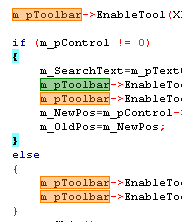
\includegraphics{incremental_search_example}

Si la chaîne de caractère recherchée ne peut pas être trouvée dans le fichier courant, afin d'indiquer que c'est ce qui se passe, le fond du masque de recherche est affiché en rouge.

\screenshot{incremental_search_settings}{Paramètres pour la Recherche Incrémentale}

\begin{description}
\item[ESC] Quitte le module de Recherche Incrémentale.
\item[ALT-Suppr] Efface l'entrée du champ de recherche incrémentale.
\end{description}

Les icônes de la barre d’outils de Recherche Incrémentale ont les significations suivantes :

\begin{description}
\item[
\includegraphics{incremental_search_clear}] Suppression du texte dans le masque de recherche de la barre d'outils de Recherche Incrémentale.
\item[
\includegraphics{incremental_search_previous},
\includegraphics{incremental_search_next}] Navigation dans les occurrences de chaîne recherchée.
\item[
\includegraphics{incremental_search_highlight}] En cliquant sur ce bouton ce sont toutes les occurrences de la chaîne recherchée qui sont surlignées en couleur, pas seulement la première.
\item[
\includegraphics{incremental_search_selected}] Activer cette option réduit le champ de recherche au passage de texte marqué dans l'éditeur.
\item[
\includegraphics{incremental_search_matchcase}] Cette option signifie que la recherche sera sensible à la casse (respect des majuscules et minuscules).
\item[
\includegraphics{incremental_search_regex}] Valider les expressions régulières dans le champ d'entrée de la recherche incrémentale.
\end{description}

\hint{Le paramétrage standard de cette barre d'outil peut être configuré dans \menu{Paramètres,Éditeur,Recherche Incrémentale}.}

%\screenshot{incremental_search_settings}{Paramètres pour la Recherche Incrémentale}

\end{INCREMENTALSEARCH}

\begin{NASSISHNEIDERMAN}
\section{Extension NassiShneiderman}\label{sec:nassishneiderman}

L'extension NassiShneiderman permet de créer des diagrammes de Nassi Shneiderman depuis \codeblocks (\cite{url:nassi}). 

\subsection{Création d'un diagramme}

Vous avez deux possibilités pour créer un diagramme.

\begin{enumerate}
\item Pour créer un diagramme vide, sélectionnez les options de menu \menu{Fichier,Nouveau,Diagramme de Nassi Shneiderman}.
\item La deuxième option consiste à créer un diagramme depuis le code source C/C++. 
\end{enumerate}

Dans une fenêtre de l'éditeur, sélectionnez une partie de code pour en créer un diagramme. Par exemple le corps d'une fonction/méthode depuis l'accolade ouvrante jusqu'à l'accolade fermante. Puis, via un clic droit sur la sélection, choisissez \menu{Nassi Shneiderman,Créer un diagramme} (voir \pxref{fig:NassiShneidermanCreate1}). 

\screenshot{NassiShneidermanCreate1}{NassiShneiderman Création}

Vous devriez obtenir un nouveau diagramme (voir \pxref{fig:NassiShneidermanCreate2}).

\screenshot{NassiShneidermanCreate2}{NassiShneiderman Exemple de Diagramme}

L'analyseur a quelques limitations:

\begin{itemize}
\item Des commentaires ne peuvent pas être placés en fin de branche.
\item Depuis la définition d'une fonction, on ne peut analyser que le corps de la fonction, pas la déclaration.
\item Bien sûr, vous en trouverez bien d'autres... 
\end{itemize}

\subsection{Édition de structogrammes}
\subsubsection{Que faire avec un diagramme ?}

Vous pouvez faire plein de choses avec un structogramme :

\begin{enumerate}
\item L'enregistrer pour l'utiliser plus tard. On peut l'enregistrer via \menu{Fichier,Enregistrer le fichier} ou \menu{Fichier,Enregistrer le fichier sous...}.
\item On peut l'exporter dans différents formats \menu{Fichier,Exporter}
    \begin{itemize}
    \item "Exporter la source..." pour l'enregistrer comme fichier source en C.
    \item "StrukTeX" pour l'utiliser dans une documentation sous LaTeX.
    \item "PNG" ou "PS" et éventuellement "SVG" pour obtenir le diagramme dans un format image connu de nombreux autres outils.
    \end{itemize}        
\item Insérer directement le code dans l'éditeur : Ouvrir ou créer un diagramme. De retour dans la fenêtre d'édition, faites un clic droit et choisissez \menu{Nassi Shneiderman,insérer en xy} (Vous obtenez ici une liste de tous les diagrammes ouverts).
\item Glisser/Déposer le diagramme (ou une partie) dans d'autres outils. Par exemple vers OpenOffice Writer afin d'y insérer une image dans votre documentation.
\end{enumerate}

Si le diagramme choisi comporte une sélection, l'exportation ou la génération de code ne portera que sur cette partie de diagramme. 

\subsubsection{Extensions}

L'extension NassiShneiderman supporte quelques extensions des diagrammes de Nassi-Shneiderman : 

\begin{itemize}
\item séparation d'une brique spécifique avec la "flèche droite"
\item continuer sur une brique spécifique avec la "flèche gauche"
\item Pour être en mesure de créer des diagrammes avec des instructions c/c++ "switch", la sélection ne doit pas être implicitement interrompue avant un "case". Les différents "cases" sont alignés verticalement. Support de C et C++.
\end{itemize}


\end{NASSISHNEIDERMAN}

\begin{LIBFINDER}
\section{LibFinder}\label{sec:lib_finder}

Si vous voulez utilisez des librairies dans votre application, vous devez configurer votre projet pour cela. Un tel processus de configuration peut être difficile et ennuyeux car chaque librairie peut utiliser un schéma d'options particulier. Un autre problème est que cette configuration diffère entre les plates-formes ce qui résulte en des incompatibilités entre des projets Unix et Windows.

LibFinder propose deux fonctionnalités majeures :

\begin{itemize}
\item Recherche des librairies installées sur votre système
\item Inclure les librairies dans votre projet en seulement quelques clics en rendant le projet indépendant de la plate-forme
\end{itemize}

\subsection{Recherche de librairies}

La recherche des librairies est disponible via le menu \menu{Extensions,Library finder}. Son but est de détecter les librairies installées sur votre système et d'enregistrer les résultats dans la base de données de LibFinder (notez que ces résultats ne sont pas écrits dans les fichiers projets de \codeblocks). La recherche commence par un dialogue où vous pouvez fournir un ensemble de répertoires où sont installées les librairies. LibFinder les analysera de façon récursive aussi, si vous ne savez pas trop où elles sont, vous pouvez sélectionner des répertoires génériques. Vous pouvez même entrer le disque complet -- dans ce cas-là, le processus de recherche prendra plus de temps mais il détectera davantage de librairies (voir \pxref{fig:list_of_directories}).

\screenshot{list_of_directories}{Liste de répertoires}

Quand LibFinder est à la recherche de librairies, il utilise des règles spéciales pour détecter leur présence. Chaque ensemble de règle est situé dans un fichier xml. Actuellement LibFinder peut rechercher wxWidgets 2.6/2.8, \codeblocks SDK et GLFW -- la liste sera étendue dans le futur.

\hint{Pour obtenir davantage de détails sur comment ajouter un support de librairie dans LibFinder, lisez dans les sources de \codeblocks \file{src/plugins/contrib/lib\_finder/lib\_finder/readme.txt}.}

Après avoir terminé l'analyse, LibFinder affiche les résultats (voir \pxref{fig:search_results}).

\screenshot{search_results}{Résultats de recherche}

Dans la liste, vous cochez les librairies qui doivent être enregistrées dans la base de données de LibFinder. Notez que chaque librairie peut avoir plus d'une configuration valide et les paramétrages ajoutés en premier sont plutôt destinés à être utilisés lors de la génération de projets.

Au-dessous de la liste, vous pouvez sélectionner ce qu'il faut faire avec les résultats des analyses précédentes :

\begin{description}
\item[Ne pas effacer les résultats précédents] Cette option travaille comme une mise à jour des résultats existants -- Cela ajoute les nouveaux et met à jour ceux qui existent déjà. Cette option n'est pas recommandée.
\item[Seconde option (Effacer les résultats précédents des librairies sélectionnées)] effacera tous les résultats des recherches précédentes des librairies sélectionnées avant d'ajouter les nouveaux résultats. C'est l'option recommandée.
\item[Effacer toutes les configurations précédentes des librairies] quand vous sélectionnez cette option, la base de données de LibFinder sera effacée avant d'y ajouter les nouveaux résultats. C'est utile quand vous voulez nettoyer une base de données LibFinder contenant des résultats invalides.
\end{description}

Une autre option de ce dialogue est \menu{Configurer les Variables Globales}. Quand vous cochez cette option, LibFinder essaiera de configurer des Variables Globales qui sont aussi utilisées pour aider à  traiter les librairies.

Si vous avez pkg-config d’installé sur votre système (C'est installé automatiquement sur la plupart des versions de systèmes linux) LibFinder proposera des librairies venant de cet outil. Il n'est pas nécessaire de faire une analyse spécifique pour celles-ci -- elles seront automatiquement chargées au démarrage de \codeblocks.

\subsection{Inclure des librairies dans les projets}

LibFinder ajoute un onglet supplémentaire dans les propriétés d'un projet \menu{Librairies} -- Cet onglet montre les librairies utilisées dans le projet ainsi que celles connues de LibFinder. Pour ajouter une librairie dans votre projet, sélectionnez là dans le panneau de droite et cliquez sur le bouton $<$. Pour enlever une librairie d'un projet, sélectionnez la dans le panneau de gauche et cliquez sur le bouton $>$ (voir \pxref{fig:project_configuration}).

\screenshot{project_configuration}{Configuration de projet}

Vous pouvez filtrer les librairies connues de LibFinder en fournissant un filtre de recherche. La case à cocher \menu{Afficher comme un arbre}  permet de basculer antre des vues sans catégories et des vues avec catégories.

Si vous voulez ajouter une librairie qui n'est pas disponible dans la base de données de LibFinder, vous pouvez utiliser le champ \menu{Librairie inconnue}. Notez que vous devriez entrer le "library's shortcode" (nom court, qui habituellement correspond au nom de variable globale) ou le nom de librairie dans pkg-config. Vous trouverez une liste de noms courts suggérés dans le Wiki de \codeblocks dans \href{http://wiki.codeblocks.org/index.php?title=Recommended_global_variables}{Global Variables}. L'usage de cette option n'est recommandé que lorsqu'on prépare un projet qui doit être généré sur d'autres machines où ce type de librairie existe et y est correctement détectée par LibFinder. Vous pouvez accéder à une variable globale dans \codeblocks comme :

\begin{lstlisting}
$(#GLOBAL_VAR_NAME.include)
\end{lstlisting}

Cocher l'option \menu{Ne pas configurer automatiquement} indiquera à LibFinder qu'il ne devrait pas ajouter automatiquement les librairies lors de la compilation. Dans ce cas, LibFinder peut s'invoquer depuis un script de génération. Un exemple d'un tel script est généré et ajouté au projet en appuyant sur  \menu{Ajouter un script de génération manuel}.

\subsection{Utilisation de LibFinder dans des projets générés par des assistants}

Les assistants vont créer des projets qui n'utilisent pas LibFinder. Pour les intégrer avec cette extension, vous devrez mettre à jour manuellement les options de génération du projet. Ceci est facilement obtenu en enlevant tous les paramétrages spécifiques aux librairies et en ajoutant les librairies au travers de l'onglet \menu{Librairies} dans les propriétés du projet.

De tels projets deviennent indépendants des plates-formes. Tant que les librairies utilisées sont dans la base de données de LibFinder, les options de génération du projet seront automatiquement mises à jour pour coïncider avec les paramétrages de librairie propres aux plates-formes.




\end{LIBFINDER}

\begin{SPELLCHECKER}
\section{Extension SpellChecker}\label{sec:spell_checker}

Une extension pour vérifier l'orthographe de chaînes de caractères et de commentaires.

\subsection{Introduction}
Une extension pour vérifier l'orthographe de chaînes de caractères et de commentaires. L'orthographe est vérifiée au cours de la frappe. De plus un thésaurus est fourni. Les deux peuvent être accédés sur demande en sélectionnant le mot en question, puis choisir entre le correcteur... ou le Thesaurus... depuis le menu d'Édition (l'opération peut être affectée à une touche d'accès rapide via le plugin Raccourcis Clavier). Le menu de contexte (clic droit sur le mot) permet d'accéder aux suggestions d'orthographe. 

\subsection{Configuration}

La configuration est dans le menu \menu{Paramêtres,Éditeur}. L'option "spell check" est à peu près à mi-chemin vers le bas de la liste de gauche.

\screenshot{ConfigureSpellChecker}{Configuration de SpellChecker}

La signification des différents contrôles est la suivante : 
\begin{description}
\item[Activer spell checker en-ligne] Active ou désactive spell checker.
\item[Langue] La langue utilisée pour la vérification orthographique et le thésaurus est sélectionnée en choisissant un dictionnaire. On peut aussi le changer dans la barre d'état.
\item[Configuration des chemins, Dictionnaires] Le plugin cherche les fichiers dictionnaires via ce chemin.
\item[Configuration des chemins, Thésaurus] Le plugin cherche les fichiers thésaurus via ce chemin.
\item[Configuration des chemins, Bitmaps] (Optionnel) Le plugin cherche, via ce chemin, les drapeaux à afficher dans la barre d'état.
\end{description}

\hint{Vous pouvez utiliser des Macros dans les trois configurations de chemins, comme par ex. \$(CODEBLOCKS)/share/codeblocks/SpellChecker. Voir Expansion de Variables pour plus de détails. Ceci est pratique si vous utilisez une version portable de \codeblocks.}

\subsection{Dictionnaires}

SpellChecker utilise une librairie nommée hunspell. Hunspell est le correcteur orthographique de OpenOffice.org, Mozilla Firefox et d'autres projets. Les dictionnaires disponibles pour ces applications sont compatibles avec ce plugin.

Open Office fourni toute une collection de dictionnaires pour plusieurs langues et dialectes à télécharger. Les extensions de OOo 3.x (*.oxt) sont des archives compressés qui peuvent être ouvertes avec votre logiciel d'archives préféré (par exemple 7-Zip ou File Roller). Copiez le fichier .aff et le fichier .dic dans le répertoire configuré dans 'Configuration des chemins, Dictionnaires' (voir ci-dessus).

Si vous êtes sous Linux vous avez sans doute déjà des dictionnaires compatibles d'installés. Regardez dans /usr/share/hunspell ou plutôt mon choix dans /usr/share/myspell/dicts. La raison pour laquelle j'aime les fichiers myspell est qu'ils incluent d'office les fichiers thésaurus qui sont correctement nommés pour travailler avec l'extension, et tout est placé au même endroit. Ne copiez pas ces fichiers. Pointez seulement spell checker vers l'endroit où ils se trouvent déjà.

Je sais que sous Windows, Firefox et Thunderbird installent aussi des fichiers dictionnaires compatibles. On peut les trouver dans... \file{C:\osp Program Files\osp Mozilla Firefox\osp dictionaries} ou \file{C:\osp Program Files\osp Mozilla Thunderbird\osp dictionaries}. De plus, OpenOffice.org et LibreOffice installent aussi des fichiers dictionnaires dans\newline
 \file{C:\osp Program Files\osp (Open/Libre)Office\osp share\osp extensions\osp dict-*}.

Le navigateur Google Chrome installe aussi des dictionnaires, mais ils sont au format .bdic et le plugin de correction orthographique de \codeblocks ne peut pas travailler avec ces fichiers.

\subsection{Fichiers Thésaurus}

Les fichiers de thésaurus sont aussi disponibles sur OOo, comme les dictionnaires. Copiez les fichiers de thésaurus (th\_*.dat and th\_*.idx) dans le répertoire configuré dans 'Configuration des chemins, Thésaurus' (voir ci-dessus) puis renommez les pour que leur nom concorde avec celui des dictionnaires mais les faire précéder de "th\_" tout en gardant l'extension telle qu'elle est.

\textbf{Exemple}: Si les fichiers dictionnaires (pour moi, une seule langue) sont "en\_GB.aff" et "en\_GB.dic" les fichiers utilisés pour le thésaurus sont "th\_en\_GB.idx" et "th\_en\_GB.dat".

Sur mon système Linux je trouve les fichiers thésaurus déjà installés dans /usr/share/myspell/dicts et /usr/share/mythes. De même, ne déplacez pas les fichiers. Configurez spell checker pour utiliser directement ces fichiers là où ils sont.

Sous Windows, si soit OpenOffice.org soit LibreOffice est installé, ils incluent souvent les fichiers thésaurus dans \file{C:\osp Program Files\osp (Open/Libre)Office\osp share\osp extensions\osp dict-*}. 

\subsection{Bitmaps (Drapeaux)}

L'image bitmap de la langue sélectionnée est affichée dans la barre d'état. S'il n'y a pas d'image bitmap, c'est le nom de la langue qui s'affiche. L'image bitmap doit être au format PNG Choisissez un drapeau dans famfamfam\_flag\_icons, copiez le dans le répertoire configuré dans 'Configuration des chemins, Bitmaps' (voir ci-dessus) et renommez-le pour que le nom soit conforme à celui du dictionnaire mais gardez l'extension png.

\subsection{Styles à vérifier}

Seul du texte possédant un style spécifique peut être vérifié (par exemple seulement des commentaires et des chaînes de caractères). Les styles sont configurés automatiquement par Scintilla (le composant d'édition de \codeblocks).

Le fichier OnlineSpellChecking.xml contient une liste avec des indices sur les styles à vérifier. Les indices ne sont pas les mêmes en fonction des langages de programmation, et donc, le fichier contient une liste pour chacun des langages de programmation. Pour ajouter des styles, regardez le nom du langage de programmation et les indices dans le fichier correspondant lexer\_*.xml puis ajoutez cette information au fichier OnlineSpellChecking.xml.

Par exemple, pour vérifier l'orthographe dans des scripts de commande bash (fichiers *.sh), ajoutez la ligne : 

\codeline{<Language name="Bash" index="2,5,6" />}

\end{SPELLCHECKER}

\begin{SRCEXPORTER}
\section{Exporter du code Source}\label{sec:src_exporter}

Il est souvent nécessaire de transférer du code source vers d'autres applications ou vers des e-mails. Si le texte est simplement copié, le formatage est perdu, ce qui rend le texte peu clair.
La fonction exporter de \codeblocks est une des solutions dans ce type de situations. Le format requis pour le fichier exporté peut être sélectionné via \menu{Fichier,Exporter}. Le programme adoptera alors le nom de fichier et le répertoire cible en fonction du fichier source ouvert et les proposera pour enregistrer le fichier à exporter. L'extension de fichier appropriée à chaque cas de figure sera déterminée par le type de l'exportation. Les formats suivants sont disponibles :

\begin{description}
\item[html] Un format de type texte qui peut être affiché dans un navigateur web ou dans un traitement de texte.
\item[rtf] Le format Rich Text qui est un format basé sur du texte et qui peut être ouvert dans un traitement de texte comme Word ou OpenOffice.
\item[odt] Le format Open Document Text qui est un format standardisé spécifié par Sun et O'Reilly. Ce format peut être traité par Word, OpenOffice et d'autres traitements de texte.
\item[pdf] Le format Portable Document qui peut être ouvert par des applications comme Acrobat Reader.
\end{description}


\end{SRCEXPORTER}

\begin{SVN}
\section{Support de SVN}\label{sec:svn}

\hint{NdT : Cette extension est traduite ici, mais est obsolète. Vous avez donc de grandes chances de ne plus la trouver dans les versions récentes de \codeblocks.}

Le support du système de contrôle de version SVN est inclus dans l'extension \codeblocks TortoiseSVN. Via le menu \menu{TortoiseSVN,Plugin settings} vous pouvez configurer les commandes svn accessibles dans l'onglet \menu{Integration}.

\begin{description}
\item[Menu intégration] Ajoute une entrée TortoiseSVN dans la barre de menu avec différents paramétrages.
\item[Project manager] Active les commandes TortoiseSVN du menu de contexte de la gestion de projet.
\item[Editor] Active les commandes TortoiseSVN du menu de contexte de l'éditeur.
\end{description}

Dans la configuration de l'extension vous pouvez choisir quelles sont les commandes svn qui sont accessibles dans le menu principal ou le menu de contexte. L'onglet intégration fournit une entrée \menu{Edit main menu} et \menu{Edit popup menu} pour paramétrer ces commandes.

\hint{L'Explorateur de fichiers dans \codeblocks utilise différentes icônes superposées afin d'indiquer l'état de svn. Les commandes de TortoiseSVN sont incluses dans le menu de contexte.}

\end{SVN}

\begin{TODOLIST}
\section{Liste des "à faire"}\label{sec:todo_list}

Dans des projets logiciels complexes, où différents développeurs sont impliqués, il est souvent nécessaire que différentes tâches soient effectuées par plusieurs utilisateurs. Pour cela, \codeblocks possède une Liste des "à faire". Cette liste s'ouvre via \menu{Affichage,Liste des "A faire"}, et contient les tâches à effectuer ensemble, avec leurs priorités, le type et le responsable de la tâche. On peut filtrer la liste par tâches, utilisateurs et/ou fichiers sources. Un tri par colonnes peut être effectué en cliquant sur le titre de la colonne correspondante.

\screenshot{todo_list}{Affichage de la Liste des "A faire"}

\hint{La liste des "à faire" peut être ajoutée à la console de messages. Sélectionnez l'option \samp{Inclure la liste des "A faire" dans le panneau de messages} à l'aide du menu \menu{Paramètres,Environnement}.}

Si les fichiers sources sont ouverts dans \codeblocks, un "à faire" peut être ajouté à la liste via la commande \samp{Ajouter un élément "à faire"} du menu de contexte. Un commentaire est ajouté dans le code sur la ligne sélectionnée.

\begin{lstlisting}
// TODO (user#1#): ajouter un nouveau dialogue pour la prochaine release
\end{lstlisting}

Quand on ajoute un "à faire", une boîte de dialogue apparaît où les paramétrages suivants peuvent être faits (voir \pxref{fig:add_todo}).

\figures[hbt!][width=.5\columnwidth]{add_todo}{Dialogue pour ajouter un "à faire"}

\begin{description}
\item[Utilisateur] Nom de l'utilisateur \var{user} pour le système d'exploitation. Les tâches pour d'autres utilisateurs peuvent également être créées ici. Pour cela, le nom de l'utilisateur correspondant doit être créé par Ajouter un nouvel utilisateur. L'assignation d'un "à faire" est alors faite via une sélection d'entrées pour cet utilisateur.

\hint{Notez que les Utilisateurs ici n'ont rien à voir avec les profils (ou personnalités) utilisés dans \codeblocks.}
\item[Type] Par défaut, le type est TODO (à faire").
\item[Priorité] Dans \codeblocks, l'importance de la tâche peut être exprimée par des priorités (1 - 9).
\item[Position] Ce paramètre spécifie si le commentaire doit être inclus avant, après ou bien à la position exacte du curseur.
\item[Style de commentaire] Une sélection de formats de commentaires (notamment doxygen).
\end{description}

\end{TODOLIST}

\begin{TOOLSPLUS}
\section{Tools+}\label{sec:tools+}

Créer un nouvel outil est assez facile, et cela peut s'effectuer en quelques étapes simples. D'abord ouvrir \menu{Tools(+),Configurer les outils...} pour accéder au dialogue des Outils définis par l'utilisateur.

\screenshot{tools_setup}{Dialogue des Outils définis par l'utilisateur}

\genterm{Nom de l'outil}

C'est le nom qui sera affiché dans le menu déroulant de Tools(+). Il sera aussi affiché comme nom d'onglet pour les Tools+ redirigés vers la fenêtre Outils.

\genterm{Ligne de Commande}

Toute ligne de commande valide, fonction et paramètres, peut être entrée ici. La substitution de variable est également acceptée. La liste suivante contient les variables les plus utiles (voir \pxref{sec:builtin_variables} pour la liste complète).

\begin{description}
\item[\$relfile, \$file] Respectivement, le nom relatif et absolu d'un fichier sélectionné.
\item[\$reldir, \$dir] Respectivement, le nom relatif et absolu d'un répertoire sélectionné.
\item[\$relpath, \$path] Le nom relatif et absolu d'un fichier ou répertoire sélectionné.
\item[\$mpaths] Une liste de fichiers ou de répertoires sélectionnés (seulement des chemins en absolu).
\item[\$fname, \$fext] Le nom sans extension et l'extension sans le nom d'un fichier sélectionné.
\item[\$inputstr\{prompt\}] Demande à l'utilisateur d'entrer une chaîne de texte qui sera substituée dans la ligne de commande.
\item[\$if(condition)\{true clause\}\{false clause\}] Résolution en \codeline{false clause} si la \codeline{condition} est vide, 0, ou fausse; sinon \codeline{true clause}.
\end{description}

\genterm{Types de fichiers}

Les expressions avec un caractère joker (*) séparées par des points virgules vont restreindre le choix par le sous-menu clic droit sur un fichier, répertoire, chemin multiple dans l'arborescence des projets, de l'explorateur de fichiers, ou du panneau d'éditeur à un/des type/s spécifiés. Laisser vide pour traiter tous les types de fichiers/répertoires.

\genterm{Répertoire de Travail}

Le répertoire sur lequel exécuter la commande. Les variables de \codeblocks, les variables de projet, et les variables globales sont disponibles. De même,

\begin{enumerate}
\item Si \codeline{\$dir} est entré dans la ligne de commande, alors \codeline{\$dir} peut aussi être utilisé ici.
\item \codeline{\$parentdir} est disponible pour \codeline{\$relfile}, \codeline{\$file}, \codeline{\$reldir}, \codeline{\$dir}, \codeline{\$relpath}, \codeline{\$path}, \codeline{\$fname}, \codeline{\$fext}, pour l'évaluation du chemin absolu d'un répertoire contenant cet élément.
\end{enumerate}

\genterm{Chemin du Menu Outils}

Contrôle l'emplacement de la commande dans le menu de Tools(+), donnant la possibilité d'ajouter des sous-menus (les niveaux multiples sont autorisés).

\begin{itemize}
  \item Submenu/Tool1
  \item Submenu/Tool2
  \item Tool3
\end{itemize}

Va créer cette structure.

\figures[H][width=.6\columnwidth]{tools_menu_path}{Structure des menus de Tools}

Le nom de la commande sera utilisé si cette entrée est vide. Si le premier caractère est un point, la commande sera cachée.

\genterm{Chemin du Menu de Contexte}

Ceci contrôle l'emplacement de la commande dans le menu clic-droit des Projets et des onglets de fichiers du panneau de Gestion. Les mêmes règles que pour la structure des menu de Tools+ s'appliquent ici.

\figures[H][width=.8\columnwidth]{tools_context_path}{Structure des menus de Contexte}

Notez SVP que la commande n'apparaîtra dans les menus de contexte que si la ligne de commande contient un ou plusieurs des éléments suivants : \codeline{\$relfile}, \codeline{\$file}, \codeline{\$reldir}, \codeline{\$dir}, \codeline{\$relpath}, \codeline{\$path}, \codeline{\$fname}, et \codeline{\$fext}.

\genterm{Sortie vers}

Ceci détermine vers où la sortie de la commande sera redirigée. Le but et la fonction de la commande détermineront ce qui est le mieux à faire.
\genterm{Tools Output Window}
Les outils qui ne requièrent que des résultats de sortie en ligne de commande (et ne demandent pas d'entrées) utilisent généralement cette façon de faire. Le programme sera lancé en mode invisible et toutes les sorties seront redirigées vers l'onglet approprié de la fenêtre de sortie des Outils Tools+. Le texte [DONE/TERMINÉ] sera ajouté en fin d'exécution de l'Outil.

\figures[H][width=.5\columnwidth]{tool_output}{Fenêtre de sortie de l'Outil}

\hint{Si la fenêtre de sortie des Outils Tools+ est ouverte à la clôture de \codeblocks, il se peut que \codeblocks plante.}

\genterm{Console de \codeblocks}
Ceci va permettre de lancer le programme via l'exécutable \file{cb\_console\_runner} (ce même programme qui est lancé après Générer et exécuter). Généralement, c'est utilisé par les outils en ligne de commande pour obtenir des interactions utilisateur avancées, bien que des programmes graphiques puissent aussi être utilisés (notamment si le programme n'est pas stable ou s'il affiche des messages dans la sortie standard). Le "Console runner" mettra la fenêtre en pause (l'empêchant de se fermer), affichera le temps d'exécution, ainsi que le code de sortie quand le programme s'arrêtera.

\genterm{Shell Standard}
C'est la même chose que de placer cette commande dans un script batch ou un script Shell puis de l'exécuter. Le programme s'exécutera quelle que soit la méthode par défaut, et lorsqu'il aura terminé, sa fenêtre se fermera.. Ce paramètre est utile pour exécuter un programme (par exemple un fichier ou un navigateur Web) qui doit rester ouvert après la fermeture de \codeblocks.

\hint{Comme le plugin Tools+ plugin est en cours de développement, quelques fonctionnalités - par exemple Priorité de Menu et Variables d'environnement - peuvent ne pas être disponibles.}

\subsection{Exemple d'Outils Tools+}

\genterm{Ouvrir l'explorateur sur un fichier sélectionné}

\begin{itemize}
\item Windows Explorer
\begin{itemize}
\item Menu Outils Tools+
\begin{verbatim}
explorer /select,"$(PROJECTFILE)"
\end{verbatim}
\item Menu de Contexte
\begin{verbatim}
explorer /select,"$path"
\end{verbatim}
\end{itemize}

\item Dolphin
\begin{itemize}
\item Menu Outils Tools+
\begin{verbatim}
dolphin --select "$(PROJECTFILE)"
\end{verbatim}
\item Menu de Contexte
\begin{verbatim}
dolphin --select "$path"
\end{verbatim}
\end{itemize}

\hint{Les trois commandes suivantes du menu contextuel ne prennent en charge que les dossiers (mais pas les fichiers).}

\item Nautilus
\begin{itemize}
\item Menu Outils Tools+
\begin{verbatim}
nautilus --no-desktop --browser "$(PROJECTDIR)"
\end{verbatim}
\item Menu de Contexte
\begin{verbatim}
nautilus --no-desktop --browser "$dir"
\end{verbatim}
\end{itemize}

\item Thunar
\begin{itemize}
\item Menu Outils Tools+
\begin{verbatim}
thunar "$(PROJECTDIR)"
\end{verbatim}
\item Menu de Contexte
\begin{verbatim}
thunar "$dir"
\end{verbatim}
\end{itemize}

\item PCMan File Manager
\begin{itemize}
\item Menu Outils Tools+
\begin{verbatim}
pcmanfm "$(PROJECTDIR)"
\end{verbatim}
\item Menu de Contexte
\begin{verbatim}
pcmanfm "$dir"
\end{verbatim}
\end{itemize}
\end{itemize}

\genterm{Mise à jour d'un répertoire Subversion}

\begin{itemize}
\item Windows
\begin{itemize}
\item Menus Outils Tools+
\begin{verbatim}
"path_to_svn\bin\svn" update "$inputstr{Directory}"
\end{verbatim}
\item Menu de Contexte
\begin{verbatim}
"path_to_svn\bin\svn" update "$dir"
\end{verbatim}
\end{itemize}

\item Linux
\begin{itemize}
\item Menus Outil Tools+
\begin{verbatim}
svn update "$inputstr{Directory}"
\end{verbatim}
\item Menu de Contexte
\begin{verbatim}
svn update "$dir"
\end{verbatim}
\end{itemize}
\end{itemize}

\genterm{Exporter un makefile}

\hint{Utilisation de l'outil en ligne de commande cbp2make.}\label{sec:tool_cbp2make}

\begin{itemize}
\item Windows
\begin{itemize}
\item Menus Outil Tools+
\begin{verbatim}
"path_to_cbp2make\cbp2make" -in "$(PROJECTFILE)"
\end{verbatim}
\end{itemize}

\item Linux
\begin{itemize}
\item Menus Outil Tools+
\begin{verbatim}
"path_to_cbp2make/cbp2make" -in "$(PROJECTFILE)"
\end{verbatim}
\end{itemize}
\end{itemize}

\genterm{Compresser le projet actif dans une archive}

\begin{itemize}
\item Windows
\begin{itemize}
\item 7z ou zip - Menus Outil Tools+ (sur 1 seule ligne)
\begin{verbatim}
"path_to_7z\7z" a -t$if(zip == $inputstr{7z or zip?}){zip -mm=Deflate
     -mmt=on -mx9 -mfb=128 -mpass=10}{7z -m0=LZMA -mx9 
     -md=64m -mfb=64 -ms=on} -sccUTF-8 "-w$(PROJECTDIR).."
     "$(PROJECTDIR)..\$(PROJECT_NAME)" "$(PROJECTDIR)*"
\end{verbatim}

\item tar.gz ou tar.bz2 - Menus Outil Tools+  (sur 1 seule ligne)
\begin{verbatim}
cmd /c ""path_to_7z\7z" a -ttar -mx0 -sccUTF-8 "-w$(PROJECTDIR).."
      "$(PROJECTDIR)..\$(PROJECT_NAME)" "$(PROJECTDIR)*" && 
      "path_to_7z\7z" a -t$if(gz == $inputstr{gz or bz2?}){gzip -mx9 
      -mfb=128 -mpass=10 -sccUTF-8 "-w$(PROJECTDIR).." 
      "$(PROJECTDIR)..\$(PROJECT_NAME).tar.gz}{bzip2 -mmt=on -mx9 
      -md=900k -mpass=7 -sccUTF-8 "-w$(PROJECTDIR).." 
      "$(PROJECTDIR)..\$(PROJECT_NAME).tar.bz2}"
      "$(PROJECTDIR)..\$(PROJECT_NAME).tar" && 
       cmd /c del "$(PROJECTDIR)..\$(PROJECT_NAME).tar""
\end{verbatim}

\hint{L'interpréteur en ligne de commande de Windows a été invoqué directement ici (\cmdline{cmd /c}), ce qui permet à des commandes multiples de s'enchaîner en une seule ligne. Cependant, cela peut provoquer un échec de l'exécution de la commande dans la console \codeblocks.}

\end{itemize}

\item Linux
\begin{itemize}
\item 7z ou zip - Menu Outils Tools+ (sur 1 seule ligne)
\begin{verbatim}
7z a -t$if(zip == $inputstr{7z or zip?}){zip -mm=Deflate -mmt=on -mx9
    -mfb=128 -mpass=10}{7z -m0=LZMA -mx9 -md=64m -mfb=64 -ms=on}
    -sccUTF-8 "-w$(PROJECTDIR).." "$(PROJECTDIR)../$(PROJECT_NAME)"
    "$(PROJECTDIR)*"
\end{verbatim}
\item tar.gz ou tar.bz2 - Menu Outils Tools+ (sur 1 seule ligne)
\begin{verbatim}
tar -cf "$(PROJECTDIR)../$(PROJECT_NAME).tar.$if(gz == $inputstr{gz 
     ou bz2?}){gz" -I 'gzip}{bz2" -I 'bzip2} -9' "$(PROJECTDIR)*"
\end{verbatim}
\end{itemize}
\end{itemize}

\end{TOOLSPLUS}

\begin{THREADSEARCH}
\section{Thread Search}\label{sec:thread_search}

Via le menu \menu{Rechercher,Thread Search}, cette extension peut être affichée ou masquée en tant qu'onglet dans la console de messages. Dans \codeblocks, une prévisualisation de l'occurrence de la chaîne de caractères peut être affichée pour un fichier, un espace de travail ou un répertoire. Ce faisant, la liste des résultats de la recherche sera affichée sur la partie droite de la console ThreadSearch. En cliquant sur une entrée de la liste, une prévisualisation s'affiche sur la partie gauche. En double-cliquant dans la liste, le fichier sélectionné est ouvert dans l'éditeur de  \codeblocks.

\hint{L'étendue des extensions de fichiers à inclure dans la recherche est préconfiguré et peut avoir besoin d'être ajusté.}

\subsection{Fonctionnalités}

L'extension ThreadSearch offre les fonctionnalités suivantes :

\begin{itemize}
\item \samp{Recherche dans les fichiers} multi tâches (Multi-threaded).
\item  Éditeur interne en lecture seule pour voir les résultats
\item Fichier ouvert dans l'éditeur de type notebook
\item Menu contextuel \samp{Rechercher les occurrences} pour commencer une recherche dans les fichiers à partir du mot situé sous le curseur
\end{itemize}

\screenshot[hbt!][width=1.1\columnwidth]{threadsearch_panel}{Panneau de Thread Search}

\subsection{Utilisation}

\begin{enumerate}
\item Configurez vos préférences de recherche (voir \pxref{fig:threadsearch_options})

Une fois l'extension installée, il y a 4 façons de conduire une recherche :

\begin{enumerate}
\item Tapez/Sélectionnez un mot dans la boîte de recherche combinée et appuyez sur Entrée ou cliquez sur Rechercher dans le panneau de Thread search de la console de messages.
\item Tapez/Sélectionnez un mot dans la boîte de recherche combinée de la barre d'outil et appuyez sur Entrée ou cliquez sur le bouton Rechercher.
\item Clic droit sur n'importe quel \samp{mot} dans l'éditeur actif puis cliquez sur \samp{Rechercher les occurrences}.
\item Cliquez sur Rechercher/Thread search pour trouver le mot courant dans l'éditeur actif.
\hint{Les points 1, 2 et 3 peuvent ne pas être disponibles en fonction de la configuration courante.}
\end{enumerate}
\item Cliquez de nouveau sur le bouton de recherche pour arrêter la recherche en cours.
\item Un clic simple sur un élément résultat l'affiche dans la prévisualisation sur la droite.
\item Un double-clic sur un élément résultat ouvre ou configure un éditeur sur la droite.
\end{enumerate}

\subsection{Configuration}

Pour accéder au panneau de configuration de l'extension ThreadSearch cliquez sur (voir \pxref{fig:threadsearch_options}) :

\screenshot{threadsearch_options}{Configuration de Thread Search}

\begin{enumerate}
\item Bouton des Options du panneau de Thread search dans la console des messages.
\item Bouton des Options dans la barre d'outils de Thread search.
\item Menu Paramètres/Environnement puis choisir l'élément Thread search dans la colonne de gauche.
\end{enumerate}

\hint{Les points 1, 2 et 3 peuvent ne pas être disponibles en fonction de la configuration courante.}

La recherche partielle défini l'ensemble de fichiers qui seront analysés.

\begin{itemize}
\item Les cases à cocher Projet et Espace de travail sont mutuellement exclusives.
\item Le chemin du répertoire peut être édité ou configuré via le bouton Sélection.
\item Masque est l'ensemble des spécifications de fichiers séparées par des \samp{;}. Par exemple: \file{*.cpp;*.c;*.h.}
\end{itemize}

\subsection{Options}

\begin{description}
\item[Mot entier] si coché, lignes contenant l'expression recherchée si l'expression recherchée est trouvée sans caractères alphanumériques \codeline{+'_'} avant et après.
\item[Début de mot] si coché, lignes contenant l'expression recherchée si l'expression recherchée est trouvée au début d'un mot sans caractères alphanumériques \codeline{+'_'} avant et après.
\item[Respecter la casse] si coché, la recherche est sensible à la casse (majuscules-minuscules).
\item[Expression régulière] l'expression recherchée est une expression régulière.
\end{description}

\hint{Si vous voulez chercher des expressions régulières comme \file{\osp n} vous devrez choisir l'option \menu{Utiliser des recherches RegEx avancées} via le menu \menu{Paramètres,Éditeur,Paramètres généraux}.}

\subsection{Options de Thread search (ou Tâche de Recherche)}

\begin{description}
\item[Activer les éléments du menu contextuel \samp{Trouver les occurrences}] Si coché, l'entrée Trouver les occurrences est ajoutée au menu contextuel de l'éditeur.
\item[Utiliser les options par défaut du menu \samp{Trouver les occurrences}] Si coché, un ensemble d'options par défaut est appliqué aux recherches lancées par \samp{Trouver les occurrences} du menu de contexte correspondant. Par défaut l'option \samp{Mot entier} et \samp{Respecter la casse} est activé.
\item[Effacer les résultats précédents en début de recherche] Si l'extension ThreadSearch est configurée en \samp{Vue arborescente} alors les résultats de la recherche sont listés dans l'ordre hiérarchique suivant,
\begin{itemize}
\item le premier noeud contient le terme cherché
\item ensuite les fichiers qui contiennent ce terme sont listés
\item dans cette liste les numéros des lignes et le contenu correspondant sont affichés
\end{itemize}
Si vous recherchez plusieurs termes, la liste deviendra confuse, aussi les résultats des recherches précédents peuvent être supprimés en utilisant cette option en début de recherche.
\hint{Dans la liste des occurrences les termes seuls ou tous les termes peuvent être supprimés via le menu de contexte \menu{Supprimer l'élément} ou \menu{Supprimer tous les éléments}.}
\end{description}

\subsection{Mise en page}

\begin{description}
\item[Afficher l'en-tête dans la fenêtre de logs] si coché, l'en-tête est affiché dans la liste des résultats de contrôle.
\hint{Si non coché, les colonnes ne sont plus redimensionnables mais on économise de la place.}
\item[Dessiner des lignes entre les colonnes] Dessine des lignes entre les colonnes en mode Liste.
\item[Afficher la barre d'outils de ThreadSearch] Afficher la barre d'outils de l'extension ThreadSearch.
\item[Afficher les widgets de recherche dans le panneau de messages de ThreadSearch] Si coché, seuls les résultats de la liste de contrôle et l'éditeur de prévisualisation sont affichés. Les autres widgets de recherches sont masqués (économise de la place).
\item[Afficher l'éditeur de prévisualisation de code] La prévisualisation du code peut être masquée soit par cette case à cocher soit par un double-clic sur la bordure du séparateur en milieu de fenêtre. C'est ici qu'on peut le faire de nouveau s'afficher.
\end{description}

\subsection{Panneau de Gestion}

Vous pouvez choisir différents modes de gestion de la fenêtre de ThreadSearch. Avec le choix \samp{Panneau de Messages} la fenêtre ThreadSearch sera intégrée à la console de messages dans un des onglets. Si vous choisissez \samp{Mise en page} vous pourrez le détacher de la console et obtenir une fenêtre flottante que vous pourrez placer ailleurs.

\subsection{Type de journal}

La vue des résultats de recherche peut s'afficher de plusieurs façons. Le choix \samp{Liste} affiche toutes les occurrences sous forme d'une liste. L'autre mode \samp{Arborescence} assemble toutes les occurrences internes d'un fichier dans un noeud.

\subsection{Mode de partage de fenêtre}

L'utilisateur peut configurer la séparation de fenêtre de prévisualisation et de sortie des résultats de recherche horizontalement ou verticalement.

\subsection{Tri des résultats de recherche}

Les résultats de recherche peuvent être triés par le nom de chemin ou le nom de fichier.

\end{THREADSEARCH}

\begin{MOREPLUGINS}
\section{Code statistics}

\screenshot{code_stats}{Configuration de Code Statistics}

Basée sur les caractéristiques d'un masque de configuration, cette simple extension détecte les pourcentages de codes, commentaires et lignes blanches d'un projet. L'évaluation se lance via la commande de menu \menu{Extensions,Code statistics}.


\section{Profilage de Code}

Une interface graphique simple au Profileur GNU GProf.


\section{Importation de Projets}

Le plugin ProjectsImporter importe des projets et des espaces de travail d'autres IDE, notamment Dev-C++, MSVC6, MSVC7, et MSVC8 pour les utiliser comme projets \codeblocks. 


\section{Recherche de Code Source Disponible}

Cette extension permet de sélectionner un terme dans l'éditeur et de rechercher ce terme à l'aide du menu de contexte \menu{Rechercher dans Koders} dans la base de données du site \cite{url:koders}. La boîte de dialogue permet d'ajouter la possibilité de filtrer les langages de programmation ou le type de licence.

\hint{Koders et son successeur BlackDuck semblent avoir disparu ou changé de site Web ! Aussi ce plugin ne fonctionne plus. En attente de mise à jour ...}

Cette recherche dans la base vous aidera à trouver du code source originaire du monde entier en provenance d'autres projets universitaires, consortiums et d'organisations comme Apache, Mozilla, Novell Forge, SourceForge et bien d'autres, qui peuvent être réutilisés sans avoir à réinventer la roue à chaque fois. SVP, regardez bien la licence du code source dans chaque cas particulier.


\section{Extension Symbol Table}

Cette extension permet de rechercher des symboles dans des fichiers objets et dans des librairies. Les options et le chemin d'accès au programme nm en ligne de commande sont définis dans l'onglet des Options.

\screenshot{symtab_config}{Configuration de Symbol Table}

Cliquer sur \samp{Rechercher} démarre la recherche. Les résultats du programme NM sont alors affichés dans une fenêtre séparée nommée \samp{SymTabs Result}. Les noms des fichiers objets et des librairies contenant les symboles sont listés avec comme titre \samp{Sortie de NM}.


\end{MOREPLUGINS}

